\documentclass[dvipdfmx,10pt,aspectratio=169]{beamer}


% figure caption
\usepackage{caption}
\captionsetup[figure]{labelformat=empty}
% font family
\usepackage{helvet}
% use gothic font for japanese
\renewcommand{\kanjifamilydefault}{\gtdefault}


% theme
\usetheme{Madrid}
\usefonttheme{professionalfonts}
\useoutertheme[height=0cm,width=1.5cm,left]{sidebar}


% frame number
\setbeamertemplate{frametitle}{
    \nointerlineskip
    \begin{beamercolorbox}[wd=\paperwidth,ht=2.25ex,dp=0.75ex]{frametitle} % set ht
        \hspace*{1ex}\insertframetitle
        % \hfill\insertframenumber/\inserttotalframenumber\hspace*{8ex}
        \hfill\insertframenumber/{27}\hspace*{8ex}
    \end{beamercolorbox}
}


% hides nvigation buttons at bottom
\setbeamertemplate{navigation symbols}{}


% Remove title and name from sidebar
\makeatletter
\setbeamertemplate{sidebar \beamer@sidebarside}%{sidebar theme}
{
    \beamer@tempdim=\beamer@sidebarwidth%
    \advance\beamer@tempdim by 10pt%
    \insertverticalnavigation{\beamer@sidebarwidth}%
    \vfill
    \ifx\beamer@sidebarside\beamer@lefttext%
    \else%
    \usebeamercolor{normal text}%
    \llap{\usebeamertemplate***{navigation symbols}\hskip0.1cm}%
    \vskip5pt%
    \fi%
}%
\makeatother


% show toc at the beginning of each section
\AtBeginSection[]
{
    \begin{frame}
        \frametitle{目次}
        \tableofcontents[currentsection]
    \end{frame}
}


% display transparently
\setbeamercovered{transparent}


% table style
% This sets the thickness of the borders of the table.
\setlength{\arrayrulewidth}{0.5mm}
% The space between the text and the left/right border of its containing cell
\setlength{\tabcolsep}{18pt}
% The height of each row is set to 1.5 relative to its default height.
\renewcommand{\arraystretch}{2.5}


% define colors
% ---------------------------------------------------------------------------- %
\definecolor{red}{rgb}{0.9,0.30,0.30}
\definecolor{blue}{rgb}{0.32,0.66,0.82}
\definecolor{darkblue}{rgb}{0.2,0.4,0.6}
\definecolor{green}{rgb}{0.47,0.72,0.29}
\definecolor{darkgreen}{rgb}{0.25,0.42,0.21}
\definecolor{yellow}{rgb}{0.95,0.85,0.25}
\definecolor{darkyellow}{rgb}{0.75,0.65,0.05}
\definecolor{orange}{rgb}{0.95,0.55,0.25}
\definecolor{darkorange}{rgb}{0.75,0.35,0.05}
\definecolor{purple}{rgb}{0.75,0.55,0.85}
\definecolor{darkpurple}{rgb}{0.55,0.35,0.65}
\definecolor{brown}{rgb}{0.75,0.55,0.25}
\definecolor{darkbrown}{rgb}{0.55,0.35,0.05}
\definecolor{pink}{rgb}{0.95,0.55,0.75}
\definecolor{darkpink}{rgb}{0.75,0.35,0.55}
\definecolor{grey}{rgb}{0.55,0.55,0.55}
\definecolor{darkgrey}{rgb}{0.35,0.35,0.35}
% ---------------------------------------------------------------------------- %


% set colors
% ---------------------------------------------------------------------------- %
\setbeamercolor{structure}{fg=blue}
\setbeamertemplate{blocks}[rounded][shadow=false]
\setbeamercolor{block title alerted}{bg=red, fg=white}
\setbeamercolor{block title example}{bg=green, fg=white}


% define blocks
% ---------------------------------------------------------------------------- %
\addtobeamertemplate{proof begin}{
    \setbeamercolor{block title}{bg=grey, fg=white}
}{}

\newenvironment<>{note}[1]{
    \setbeamercolor{block title}{bg=blue, fg=white}
    \begin{block}{Note}#1}{\end{block}}
\newenvironment<>{warning}[1]{
    \setbeamercolor{block title}{bg=red}
    \begin{block}{Warning}#1}{\end{block}}
\newenvironment<>{important}[1]{
    \setbeamercolor{block title}{bg=orange}
    \begin{block}{Important}#1}{\end{block}}

\newenvironment<>{theorem}[1]{
    \setbeamercolor{block title}{bg=darkblue, fg=white}
    \begin{block}{定理}#1}{\end{block}}
% \newenvironment<>{proof}[1]{
%     \setbeamercolor{block title}{bg=grey, fg=white}
%     \begin{block}{証明は論文}#1}{\end{block}}
\newenvironment<>{definition}[1]{
    \setbeamercolor{block title}{bg=grey}
    \begin{block}{定義}#1}{\end{block}}
% \newenvironment<>{definition}[1]{
%     \setbeamercolor{block title}{bg=grey}
%     \begin{block}{Definition}#1}{\end{block}}
\newenvironment<>{proposition}[1]{
    \setbeamercolor{block title}{bg=darkblue}
    \begin{block}{Proposition}#1}{\end{block}}
\newenvironment<>{lemma}[1]{
    \setbeamercolor{block title}{bg=darkblue}
    \begin{block}{Lemma}#1}{\end{block}}
\newenvironment<>{corollary}[1]{
    \setbeamercolor{block title}{bg=darkblue}
    \begin{block}{Corollary}#1}{\end{block}}
\newenvironment<>{remark}[1]{
    \setbeamercolor{block title}{bg=blue}
    \begin{block}{Remark}#1}{\end{block}}
% ---------------------------------------------------------------------------- %
% mathtools: math tools, mathrsfs: RSFS fonts
\usepackage{mathtools,mathrsfs}
% physics
\usepackage{physics}
% algorithm
\usepackage{algorithm,algorithmic}
% vector graphics
\usepackage{tikz}
\usetikzlibrary{quantikz}
% comment
\usepackage{comment}
% dummy text
\usepackage{lipsum}
% image position
\usepackage{here}


% latin abbreviations
% ---------------------------------------------------------------------------- %
\newcommand{\etal}{\textit{et al.}}
\newcommand{\eg}{\textit{e.g.}}
\newcommand{\cf}{\textit{c.f.}}
\newcommand{\ie}{\textit{i.e.}}
\newcommand{\etc}{\textit{etc.}}
% ---------------------------------------------------------------------------- %


% math
% ---------------------------------------------------------------------------- %
% mathbb
\newcommand{\bbA}{\mathbb{A}}
\newcommand{\bbB}{\mathbb{B}}
\newcommand{\bbC}{\mathbb{C}}
\newcommand{\bbD}{\mathbb{D}}
\newcommand{\bbE}{\mathbb{E}}
\newcommand{\bbF}{\mathbb{F}}
\newcommand{\bbG}{\mathbb{G}}
\newcommand{\bbH}{\mathbb{H}}
\newcommand{\bbI}{\mathbb{I}}
\newcommand{\bbJ}{\mathbb{J}}
\newcommand{\bbK}{\mathbb{K}}
\newcommand{\bbL}{\mathbb{L}}
\newcommand{\bbM}{\mathbb{M}}
\newcommand{\bbN}{\mathbb{N}}
\newcommand{\bbO}{\mathbb{O}}
\newcommand{\bbP}{\mathbb{P}}
\newcommand{\bbQ}{\mathbb{Q}}
\newcommand{\bbR}{\mathbb{R}}
\newcommand{\bbS}{\mathbb{S}}
\newcommand{\bbT}{\mathbb{T}}
\newcommand{\bbU}{\mathbb{U}}
\newcommand{\bbV}{\mathbb{V}}
\newcommand{\bbW}{\mathbb{W}}
\newcommand{\bbX}{\mathbb{X}}
\newcommand{\bbY}{\mathbb{Y}}
\newcommand{\bbZ}{\mathbb{Z}}

% \mathrm capital letters
\newcommand{\rmA}{\mathrm{A}}
\newcommand{\rmB}{\mathrm{B}}
\newcommand{\rmC}{\mathrm{C}}
\newcommand{\rmD}{\mathrm{D}}
\newcommand{\rmE}{\mathrm{E}}
\newcommand{\rmF}{\mathrm{F}}
\newcommand{\rmG}{\mathrm{G}}
\newcommand{\rmH}{\mathrm{H}}
\newcommand{\rmI}{\mathrm{I}}
\newcommand{\rmJ}{\mathrm{J}}
\newcommand{\rmK}{\mathrm{K}}
\newcommand{\rmL}{\mathrm{L}}
\newcommand{\rmM}{\mathrm{M}}
\newcommand{\rmN}{\mathrm{N}}
\newcommand{\rmO}{\mathrm{O}}
\newcommand{\rmP}{\mathrm{P}}
\newcommand{\rmQ}{\mathrm{Q}}
\newcommand{\rmR}{\mathrm{R}}
\newcommand{\rmS}{\mathrm{S}}
\newcommand{\rmT}{\mathrm{T}}
\newcommand{\rmU}{\mathrm{U}}
\newcommand{\rmV}{\mathrm{V}}
\newcommand{\rmW}{\mathrm{W}}
\newcommand{\rmX}{\mathrm{X}}
\newcommand{\rmY}{\mathrm{Y}}
\newcommand{\rmZ}{\mathrm{Z}}

% \mathcal capital letters
\newcommand{\calA}{\mathcal{A}}
\newcommand{\calB}{\mathcal{B}}
\newcommand{\calC}{\mathcal{C}}
\newcommand{\calD}{\mathcal{D}}
\newcommand{\calE}{\mathcal{E}}
\newcommand{\calF}{\mathcal{F}}
\newcommand{\calG}{\mathcal{G}}
\newcommand{\calH}{\mathcal{H}}
\newcommand{\calI}{\mathcal{I}}
\newcommand{\calJ}{\mathcal{J}}
\newcommand{\calK}{\mathcal{K}}
\newcommand{\calL}{\mathcal{L}}
\newcommand{\calM}{\mathcal{M}}
\newcommand{\calN}{\mathcal{N}}
\newcommand{\calO}{\mathcal{O}}
\newcommand{\calP}{\mathcal{P}}
\newcommand{\calQ}{\mathcal{Q}}
\newcommand{\calR}{\mathcal{R}}
\newcommand{\calS}{\mathcal{S}}
\newcommand{\calT}{\mathcal{T}}
\newcommand{\calU}{\mathcal{U}}
\newcommand{\calV}{\mathcal{V}}
\newcommand{\calW}{\mathcal{W}}
\newcommand{\calX}{\mathcal{X}}
\newcommand{\calY}{\mathcal{Y}}
\newcommand{\calZ}{\mathcal{Z}}

% multiplicative group
\newcommand{\Zx}{\Z^\times}
\newcommand{\Qx}{\Q^\times}
\newcommand{\Rx}{\R^\times}
\newcommand{\Cx}{\C^\times}

% non-negative
\newcommand{\Znn}{\Z_{\ge0}}
\newcommand{\Qnn}{\Q_{\ge0}}
\newcommand{\Rnn}{\R_{\ge0}}

% positive
\newcommand{\Zpo}{\Z_{>0}}
\newcommand{\Qpo}{\Q_{>0}}
\newcommand{\Rpo}{\R_{>0}}

% mathrm
\newcommand{\const}{\mathrm{const}}
\newcommand{\hc}{\mathrm{h.c.}}
\newcommand{\lhs}{\mathrm{(LHS)}}
\newcommand{\rhs}{\mathrm{(RHS)}}
\newcommand{\Haar}{\mathrm{Haar}}
\newcommand{\poly}{\mathrm{poly}}
\newcommand{\SWAP}{\mathrm{SWAP}}

% MathOperator
\DeclareMathOperator*{\argmin}{arg~min}
\DeclareMathOperator*{\argmax}{arg~max}
\DeclareMathOperator{\sgn}{sgn}
\DeclareMathOperator{\sign}{sign}
\DeclareMathOperator{\Supp}{Supp}
\DeclareMathOperator{\diag}{diag}
\DeclareMathOperator{\E}{E}
\DeclareMathOperator{\Var}{Var}
\DeclareMathOperator{\Cov}{Cov}
\DeclareMathOperator{\Hom}{Hom}
\DeclareMathOperator{\Aut}{Aut}
\DeclareMathOperator{\End}{End}

% others
\renewcommand{\bar}[1]{\overline{#1}}
\newcommand{\combi}[2]{{}_{#1}\text{C}_{#2}}
\newcommand{\dg}{^\dagger}
\newcommand{\fa}{{}^\forall}
\newcommand{\ex}{{}^\exists}
\newcommand{\pd}{\partial}
\newcommand*\circled[1]{\tikz[baseline=(char.base)]{
            \node[shape=circle,draw,inner sep=2pt] (char) {#1};}\,}
\newcommand{\bs}[1]{\vb*{#1}}
\newcommand{\bx}{\vb*{x}}
\newcommand{\by}{\vb*{y}}
\newcommand{\bth}{\vb*{\theta}}
\newcommand{\ot}{\otimes}
\newcommand{\otn}[1]{^{\otimes {#1}}}
\newcommand{\kten}[2]{\ket{#1}\otimes\ket{#2}}
\newcommand{\bten}[2]{\bra{#1}\otimes\bra{#2}}
\newcommand{\memo}[1]{\textcolor{red}{(#1)}}
\usepackage{dsfont}
\newcommand{\bbid}{\mathds{1}}
% ---------------------------------------------------------------------------- %


% physics
% ---------------------------------------------------------------------------- %
% matrix
\newcommand{\paulix}{ \mqty(\pmat{1}) }
\newcommand{\pauliy}{ \mqty(\pmat{2}) }
\newcommand{\pauliz}{ \mqty(\pmat{3}) }

\newcommand{\rx}[1]{ \mqty[\cos \frac{#1}{2} & -i\sin\frac{#1}{2} \\ -i\sin \frac{#1}{2}& \cos\frac{#1}{2} ]}
\newcommand{\ry}[1]{ \mqty[\cos \frac{#1}{2} & -\sin\frac{#1}{2}  \\ \sin \frac{#1}{2}  & \cos\frac{#1}{2} ]}
\newcommand{\rz}[1]{ \mqty[e^{-i{#1}/2}      & 0                  \\ 0                  & e^{i{#1}/2}     ]}
\newcommand{\rot}[1]{\mqty[\cos {#1}         & -\sin {#1}         \\ \sin {#1}          & \cos {#1} ]}

% sin cos
\newcommand{\sif}[2]{\sin\qty(\frac{#1}{#2})}
\newcommand{\cof}[2]{\cos\qty(\frac{#1}{#2})}

% spin
\newcommand{\up}{\uparrow} %spin up
\newcommand{\down}{\downarrow} %spin down
\newcommand{\szero}{\mqty( 1 \\ 0 )} %spin zero
\newcommand{\sone}{\mqty( 0 \\ 1 )} %spin one
% ---------------------------------------------------------------------------- %

% ref: https://github.com/SSoelvsten/latex-preamble-and-examples/tree/main/documents
\graphicspath{{../img/}}


\title{Analysis of Data-encoding Induced Barren Plateau in Quantum Machine Learning}
\author{Kensuke Kamisoyama}
\date{2024/01/24}

\begin{document}

\frame{\titlepage}

\begin{frame}{Contents}
    \tableofcontents
\end{frame}



\section{Background Knowledge}

\subsection{Quantum Computers}
\begin{frame}{Quantum Computers}
    \begin{center}
        {\large\colorbox{blue!40}{\makebox[15em]{Quantum Computers}}}
    \end{center}
    \begin{center}
        \begin{minipage}{0.9\textwidth}
            Quantum circuits consist of the following elements:
            \begin{itemize}
                \item Quantum Bits (Qubits): Two-level quantum systems
                \item Quantum Gates: Unitaries that change the state of qubits
                \item Measurements: Extract information from the quantum state
            \end{itemize}
        \end{minipage}
    \end{center}

    \begin{center}
        {\large\colorbox{blue!40}{\makebox[27em]{NISQ (Noisy Intermediate-Scale Quantum device) {\small[\href{http://arxiv.org/abs/1801.00862}{Preskill2018}]} }}}
    \end{center}

    \begin{center}
        \begin{minipage}{0.8\textwidth}
            \begin{itemize}
                \item Quantum computers with a few hundred qubits
                \item Unable to perform error correction, so noise cannot be ignored
                \item Limited depth of quantum circuits
            \end{itemize}
        \end{minipage}
    \end{center}
\end{frame}



\newcommand{\tabitem}{\usebeamertemplate{itemize item}\hspace*{\labelsep}}
\subsection{Variational Quantum Algorithms (VQA)}
\begin{frame}{Variational Quantum Algorithms (VQA)}
    \vspace*{-5pt}
    \begin{center}
        {\large\colorbox{blue!40}{\makebox[17em]{Variational Quantum Algorithms (VQA)} {\small[\href{http://arxiv.org/abs/2012.09265}{review:Cerezo2021}]} }}
    \end{center}

    \begin{center}
        \begin{minipage}{1\textwidth}
            \begin{itemize}
                \item Quantum and classical hybrid algorithms feasible on NISQ devices
                \item $U(\bth)$: Parameterized quantum circuit (variational quantum circuit)
                \item $\ell_{i,k}(\bth) = \Tr[U(\bth)\rho_i U\dg(\bth)O_k]$, where $\rho_i$ is the initial state, $O_k$ is the observable
                \item Optimization of cost function $\calL(\bth) = f(\{\ell_{i,k}(\bth)\}_{i,k})$
                \item Applications in quantum chemistry, combinatorial optimization, machine learning.
            \end{itemize}
        \end{minipage}
    \end{center}

    \centering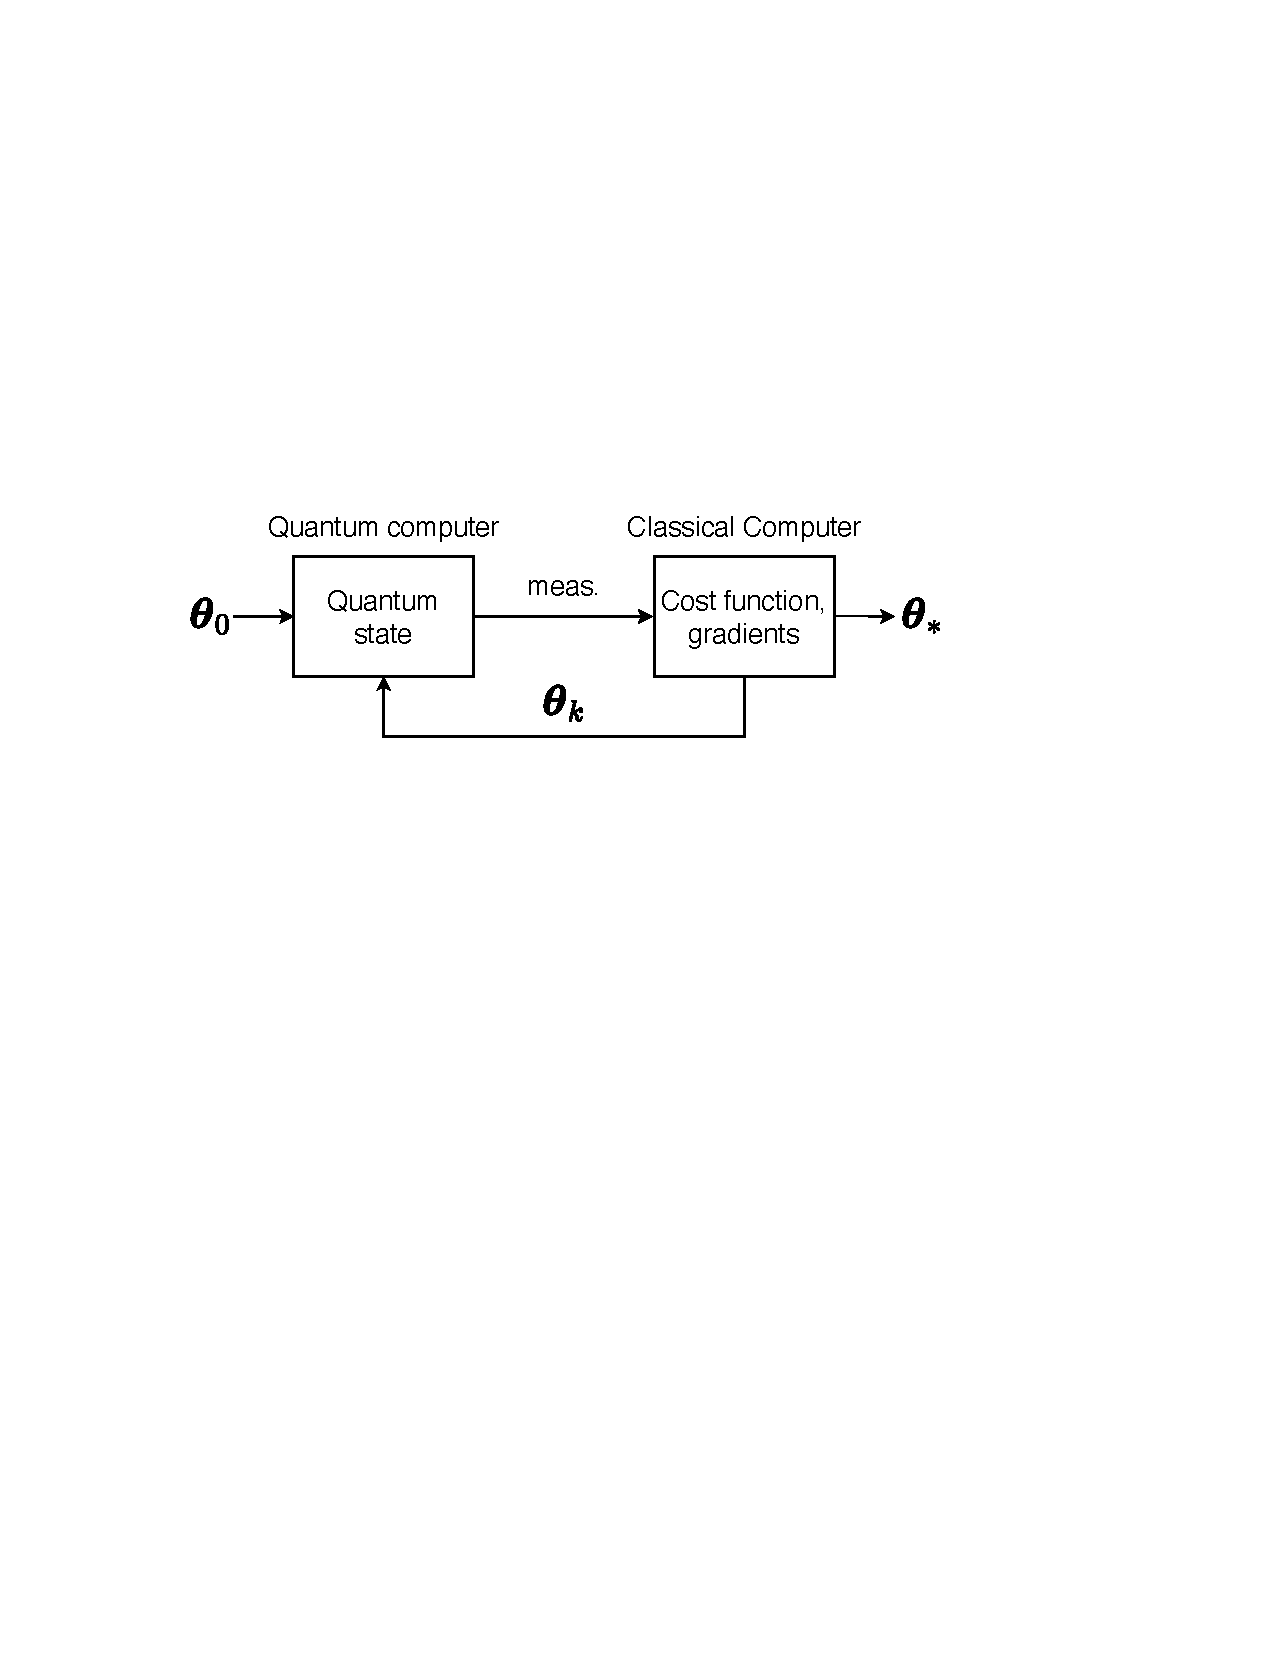
\includegraphics[width=9cm]{vqa-flow-en.pdf}
\end{frame}



\subsection{Quantum Machine Learning}

\newcommand{\encdash}{\gategroup[3,steps=1,style={inner sep=-5pt},background,label style={label position=below,anchor=north,yshift=-0.3cm}]{Encoding}}
\newcommand{\ansdash}{\gategroup[3,steps=1,style={inner sep=-5pt},background,label style={label position=below,anchor=north,yshift=-0.3cm}]{Ansatz}}

\begin{frame}{Quantum Machine Learning}
    Here, we refer to machine learning using variational quantum circuits as \textcolor{blue}{Quantum Machine Learning}. In supervised quantum machine learning, an \textcolor{blue}{encoding circuit} for the dataset $\{\bx_i,\by_i\}_i$ is necessary.

    \begin{center}
        {\large\colorbox{blue!40}{\makebox[30em]{Supervised Learning (Quantum Circuit Learning Model {\small[\href{http://arxiv.org/abs/1803.00745}{Mitarai2018}]} )}}}
    \end{center}
    \begin{columns}
        \begin{column}{0.5\textwidth}
            \centering
            Trial function\\
            $\ket{\phi(\bx_i,\bth)} := V(\bth)U(\bx_i)\ket{0}^{\otimes n}$\\
            \vspace*{10pt}
            Predicted label\\
            $\ell_{i}(\bth) := \expval{O}{\phi(\bx_i,\bth)}$\\
            \vspace*{10pt}
            Cost function\\
            $\calL(\bth) := \frac1N\sum_{i=1}^N f(y_i,\ell_{i}(\bth))$
        \end{column}

        \begin{column}{0.5\textwidth}
            \begin{center}
                \begin{tikzpicture}
                    \node[scale=1]{
                        \begin{quantikz}
                            \lstick{$\ket{0}$} & \gate[wires=3,bundle={2},style={fill=cyan!50}]{U(\bx_i)}\encdash & \gate[wires=3,bundle={2},style={fill=red!50}]{V(\bth)}\ansdash & \meter{} \\
                            \lstick{$\vdots$}  & & & {\;\vdots}\qwbundle[alternate]{}\\
                            \lstick{$\ket{0}$} & & & \meter{}
                            % & \text{Encoding} & \text{Ansatz} & \\
                        \end{quantikz}
                        };
                \end{tikzpicture}
            \end{center}
        \end{column}
    \end{columns}
    
\end{frame}



\subsection{Barren Plateau (BP)}
\begin{frame}{Barren Plateau (BP)}
    \begin{columns}
        \vspace*{-50pt}
        \begin{column}{0.65\textwidth}
            \begin{center}
                {\large\colorbox{blue!40}{\makebox[17em]{Barren Plateau {\small[\href{http://arxiv.org/abs/1803.11173}{Mcclean2018}]}}}}
            \end{center}
            \vspace*{-10pt}
            \begin{definition}
                $\calL(\bs{\theta})$: Cost function, $V(\bs{\theta})$: Ansatz, $n$: Number of qubits
                $$\E_{V(\bth)}\left[\frac{\pd \calL(\bth)}{\pd \theta_\nu}\right] = 0, \,\,\Var_{V(\bth)}\left[\frac{\pd \calL(\bth)}{\pd \theta_\nu}\right] \in \calO(2^{-\alpha n}), \,\,\alpha > 0 $$
            \end{definition}
            Gradient vanishing → Exponential complexity\\
             \textcolor{blue}{Scaling of the variance of gradient} is important
            \begin{center}
                \begin{tikzpicture}[scale=0.8]
                    \def\a{1}
                    \def\b{0.8}
                    \def\c{0.1}
                    \def\d{2.2}
                    \draw [domain=0:4,smooth] plot (\x,{-2*\b^2/(\b^2 + (\x-2)^2) + \d});
                    \draw [domain=5:9,smooth] plot (\x,{-2*\c^2/(\c^2 + (\x-7)^2) + \d});
                    \draw [->,thick] (0,2.7) -- (9.5,2.7) node [right]{$n$};
                    \draw [->] (0,0) -- (4,0) node [right]{$\theta_\nu$};
                    \draw [->] (5,0) -- (9,0) node [right]{$\theta_\nu$};
                \end{tikzpicture}
            \end{center}
        \end{column}

        \begin{column}{0.35\textwidth}
            {\large Causes}
            \begin{itemize}
                \item Depth of the ansatz
                \item Locality of observables
                \item Noise
                \item \textcolor{blue}{Data encoding}
            \end{itemize}

            \begin{figure}
                \centering
                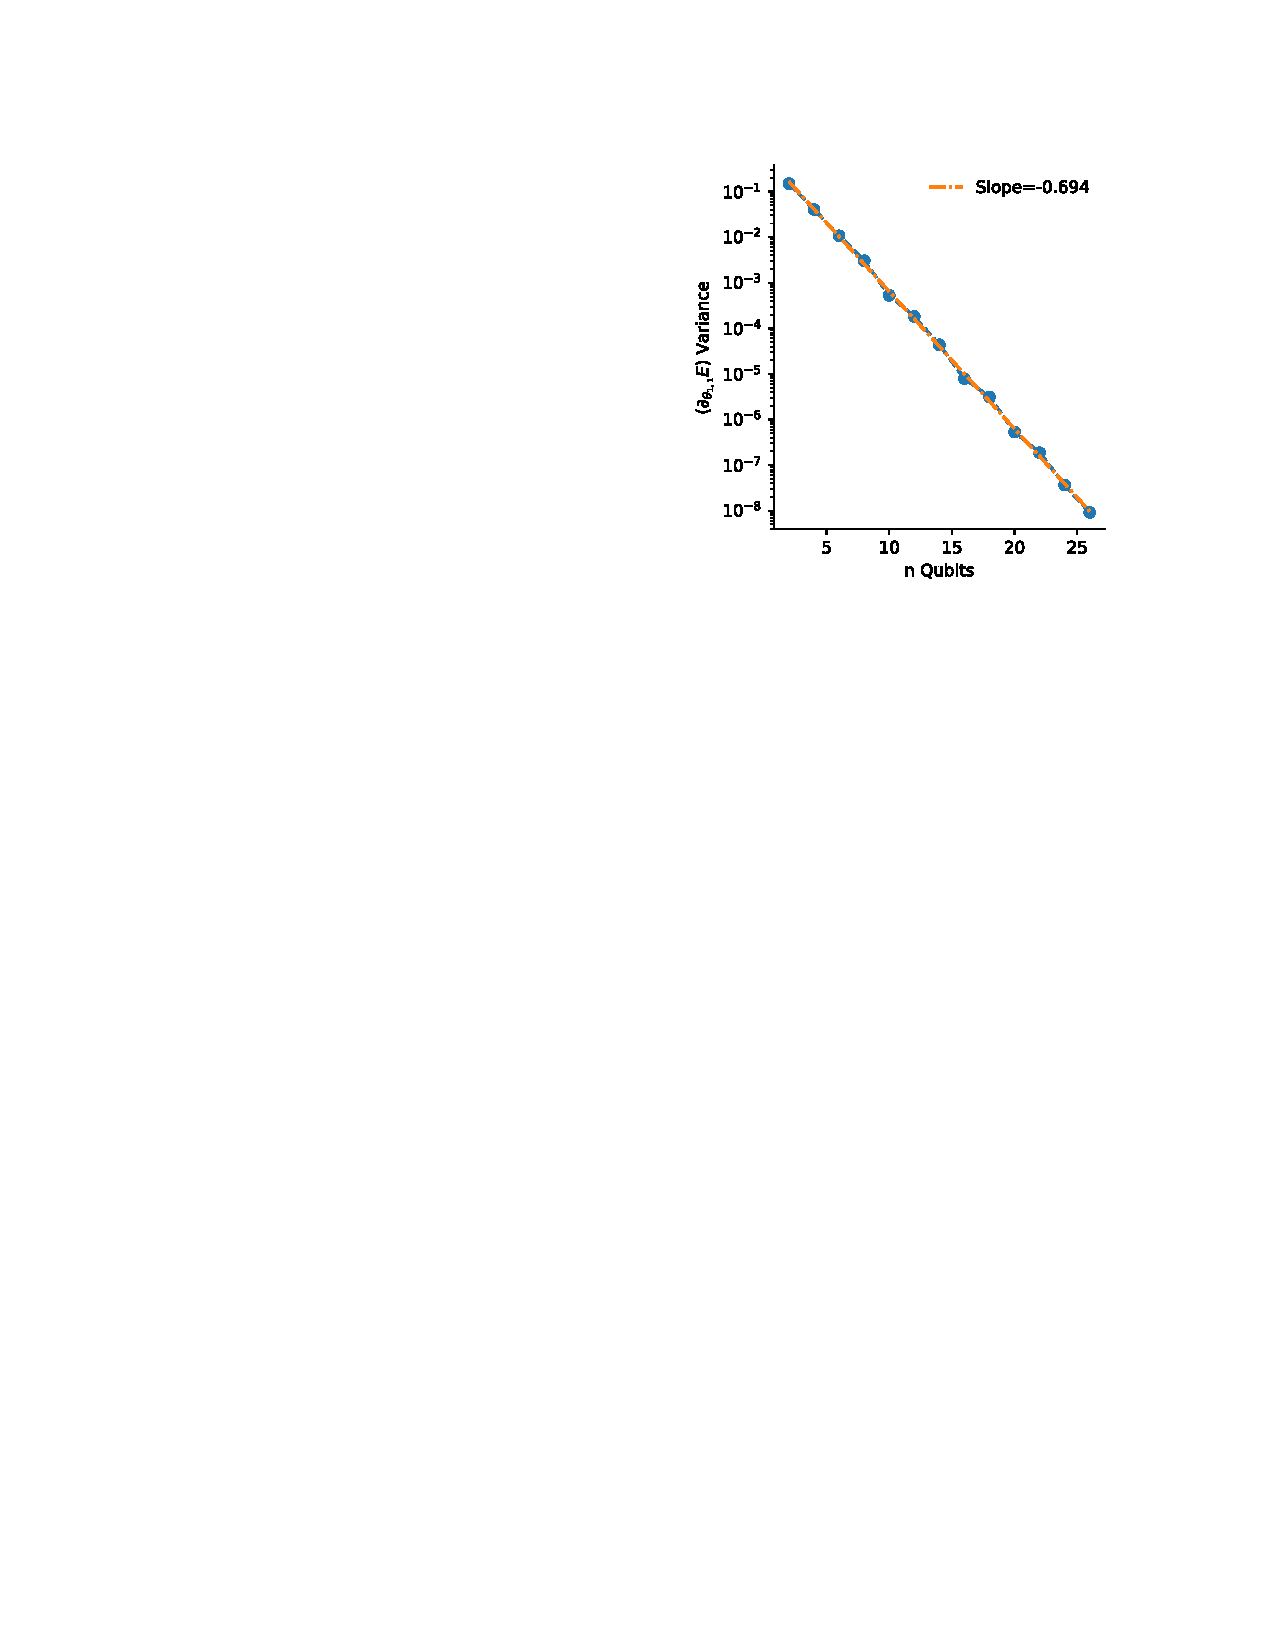
\includegraphics[height=4cm,width=4cm]{bp-var.pdf}
                \vspace*{-5pt}
                \caption{Variance of cost function gradient}
            \end{figure}
        \end{column}
    \end{columns}
\end{frame}



\section{Research Overview}
\begin{frame}{Research Overview}
    \begin{center}
        {\large\colorbox{blue!40}{\makebox[15em]{Research Background}}}
    \end{center}
    \begin{center}
        \begin{minipage}{0.9\textwidth}
            \begin{itemize}
                \item make machine learning efficient using variational quantum algorithms
                \item However, Barren Plateau (gradient vanishing) may arise
                \item Additionally, the effect of data encoding has not been investigated well
            \end{itemize}
        \end{minipage}
    \end{center}

    \begin{center}
        {\large\colorbox{blue!40}{\makebox[15em]{Research Goal and Approaches}}}
    \end{center}

    Goal: To prevent the Barren Plateau due to data encoding\\
    
    Approach: 
    \begin{center}
        \begin{minipage}{1\textwidth}
            \begin{enumerate}
                \item Analyze the effect of data encoding on the variance of the cost function gradient. Specifically, we derive upper and lower bounds on the variance of gradient.
                \item Numerically verify that the scaling of the variance of gradient is independent of the forms of the cost function.
            \end{enumerate}
        \end{minipage}
    \end{center}
\end{frame}



\section{Upper Bound on the Variance of Gradient}
\begin{frame}{Upper Bound on the Variance of the Gradient: Setup}
    \centering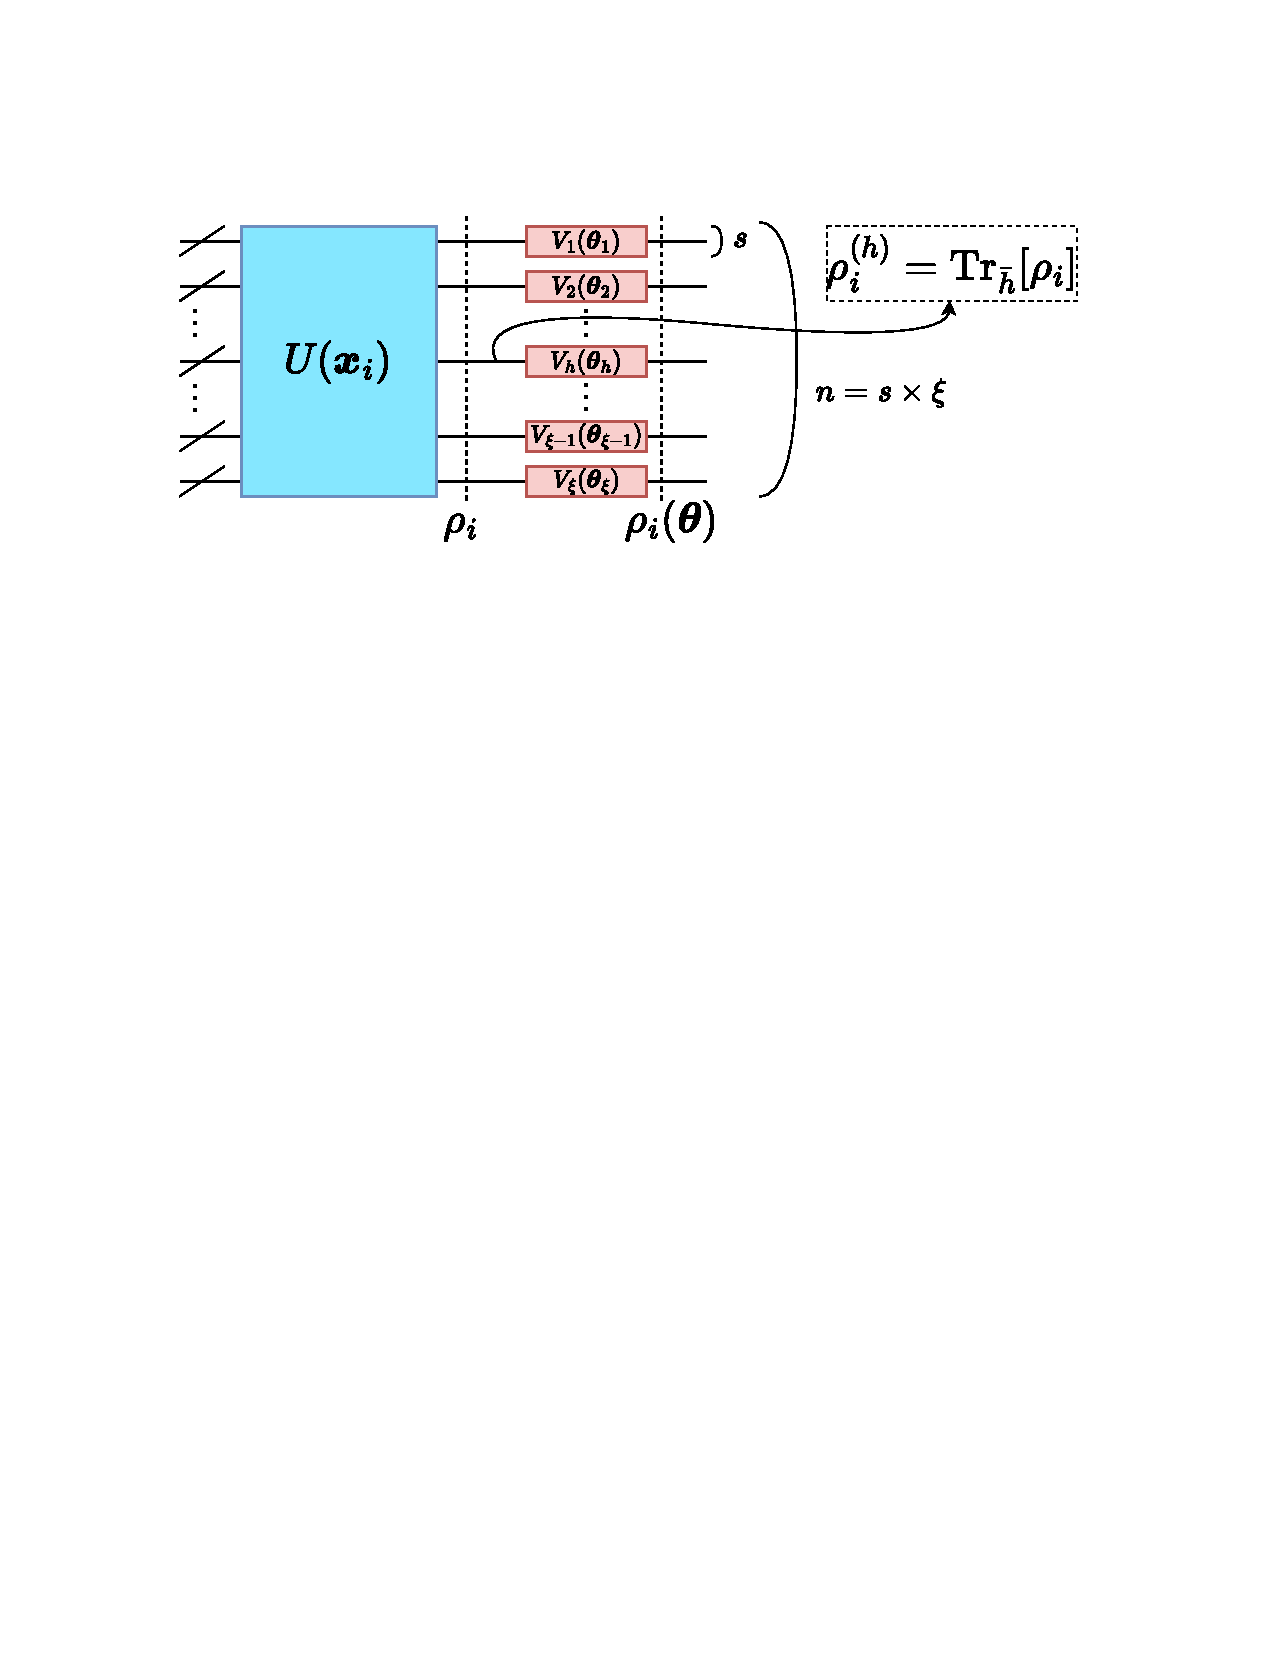
\includegraphics[width=12cm]{setting.pdf}
    $$
    \colorbox{orange!30}{$\ell_i(\bth)$} = \Tr[\rho_i(\bth)\,O_L] \in [0,1],
    \quad
    O_L=\frac1n \sum_{j=1}^{n}\dyad{0}_{j} \otimes \bbid_{\bar{j}}
    $$\\
    \vspace*{5pt}
    Set the ansatz and $O_L$ so that Barren Plateau does not occur due to factors other than data encoding.
\end{frame}



\begin{frame}{Upper Bound on the Variance of the Gradient: Results}
    \vspace*{-15pt}
    $$y_i \in \{0,1\},\quad \colorbox{orange!30}{$\ell_i(\bth)$} := \Tr[\rho_i(\bth)\,O_L] \in [0,1],\quad
    \colorbox{green!30}{$\calL(\bth)$} := \frac1N\sum_{i=1}^N f(y_i, \colorbox{orange!30}{$\ell_i(\bth)$})$$
    \vspace*{-5pt}
    Based on prior research{\small[\href{https://arxiv.org/abs/2110.14753v1}{Thanasilp2021}]}, we derived a new upper bound.

    \begin{theorem}
        Upper bound on the variance of the cost function gradient is given as follows, where $\bbU := \{U(\bs{x})|\,\bs{x}\in \calX\}$:
        \vspace*{-10pt}
        \begin{align*}
            \Var_{V(\bth)}[\pd_{\theta_\nu} \colorbox{green!30}{$\calL(\bth)$}] \;\;
            \leq\;\;
            A_f \times r_{n,s} \times \bar{D}_{\mathrm{HS}}^s \;\;
            \leq\;\;
            A_f \times r_{n,s} \times \qty(\frac{2^s-2^{-s}}{2^n+1} + \epsilon_{\bbU})
        \end{align*}
    \end{theorem}

    \begin{itemize}
        \item $A_f$ is a term depending on the function $f$ such as squared error.
        \item $r_{n,s}$ is a term depending on the observable being measured.
        \item $\bar{D}_{\mathrm{HS}}^s := \int_{\bbU}dU D_{\mathrm{HS}} ( \rho^{(h)} ,\, \bbid/2^s )$ is a term depending on the data encoding.
        \item $\epsilon_{\bbU}$ is a measure of the expressive power of the encoding circuit, and the higher the expressive power, the smaller this value is.
    \end{itemize}

    Assuming $\epsilon_{\bbU}$ does not go to $0$,
    we analyzed the scaling of $\bar{D}_{\mathrm{HS}}^s$
\end{frame}




\newcommand{\bgbs}[1]{\gate[wires=2,style={fill=cyan!50}][1cm][0.1cm]{}\slice{#1}}
\newcommand{\bgb}{\gate[wires=2,style={fill=cyan!50}][1cm][0.1cm]{}}
\newcommand{\agb}{\gate[wires=1,style={fill=red!50}][1cm][0.5cm]{}}
\begin{frame}{Upper Bound on the Variance of the Gradient: Circuit}
    Assuming the following Alternating Layered Ansatz (ALT) for the encoding circuit $U(\bx)$, we exactly calculated $\bar{D}_{\mathrm{HS}}^{s=1}$ ${}^\text{*}$
    \begin{figure}[H]
        \centering
        \begin{tikzpicture}
            \node[scale=0.7]{
            \begin{quantikz}
                \qw &\bgbs{1}& \qw     &\bgbs{3}& \qw     & \bgbs{5}& \agb & \qw\\[-0.3cm]
                \qw & \qw    & \bgbs{2}& \qw    & \bgbs{4}& \qw     & \agb & \qw\\[-0.3cm]
                \qw & \bgb   & \qw     & \bgb   & \qw     & \bgb    & \agb & \qw\\[-0.3cm]
                \qw & \qw    & \bgb    & \qw    & \bgb    & \qw     & \agb & \qw\\[-0.3cm]
                \qw & \bgb   & \qw     & \bgb   & \qw     & \bgb    & \agb & \qw\\[-0.3cm]
                \qw & \qw    & \bgb    & \qw    & \bgb    & \qw     & \agb & \qw\\[-0.3cm]
                \qw & \bgb   & \qw     & \bgb   & \qw     & \bgb    & \agb & \qw\\[-0.3cm]
                \qw & \qw    & \qw     & \qw    & \qw     & \qw     & \agb & \qw
            \end{quantikz}
            };
        \end{tikzpicture}
        \caption{Blue represents the encoding circuit, and red represents the ansatz.}
        \label{fig:alt-tpa-structure}
    \end{figure}

    \begin{scriptsize}
        (*Each blue block is treated as unitary $2$-design, and calculations were performed using the Random Tensor Network Integrator (RTNI) [\href{http://arxiv.org/abs/1902.08539}{Fukuda2019}])
    \end{scriptsize}
\end{frame}





\begin{frame}{Variance of gradient and Its Upper Bound}\label{qml-var-alt}
    \begin{columns}
        \begin{column}{0.5\textwidth}
            \centering $\Var_{V(\bth)}[\pd_{\theta_\nu} \calL(\bth)]$
            \vspace{-10pt}
            \begin{figure}
                \centering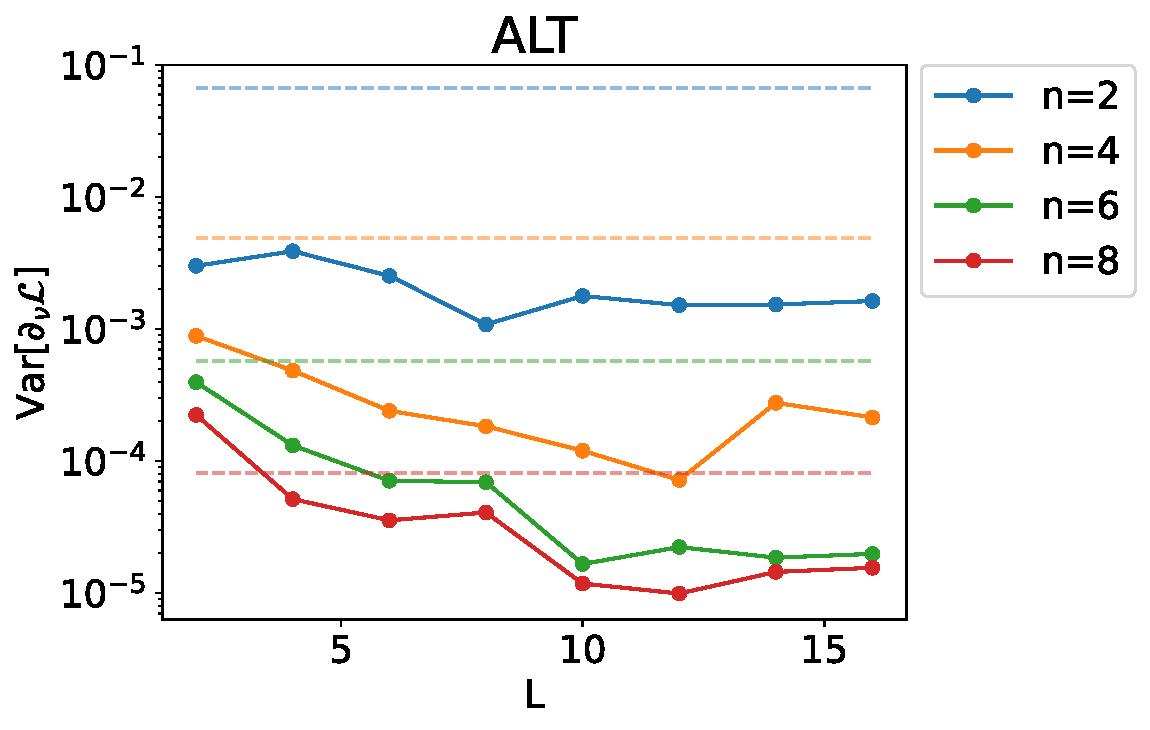
\includegraphics[width=7cm]{qml-var-alt.pdf}
            \end{figure}
        \end{column}
        \begin{column}{0.5\textwidth}
            \centering Upper Bound ($A_f \times r_{n,s} \times \bar{D}_{\mathrm{HS}}^{s=1}$)
            \vspace{-10pt}
            \begin{figure}
                \centering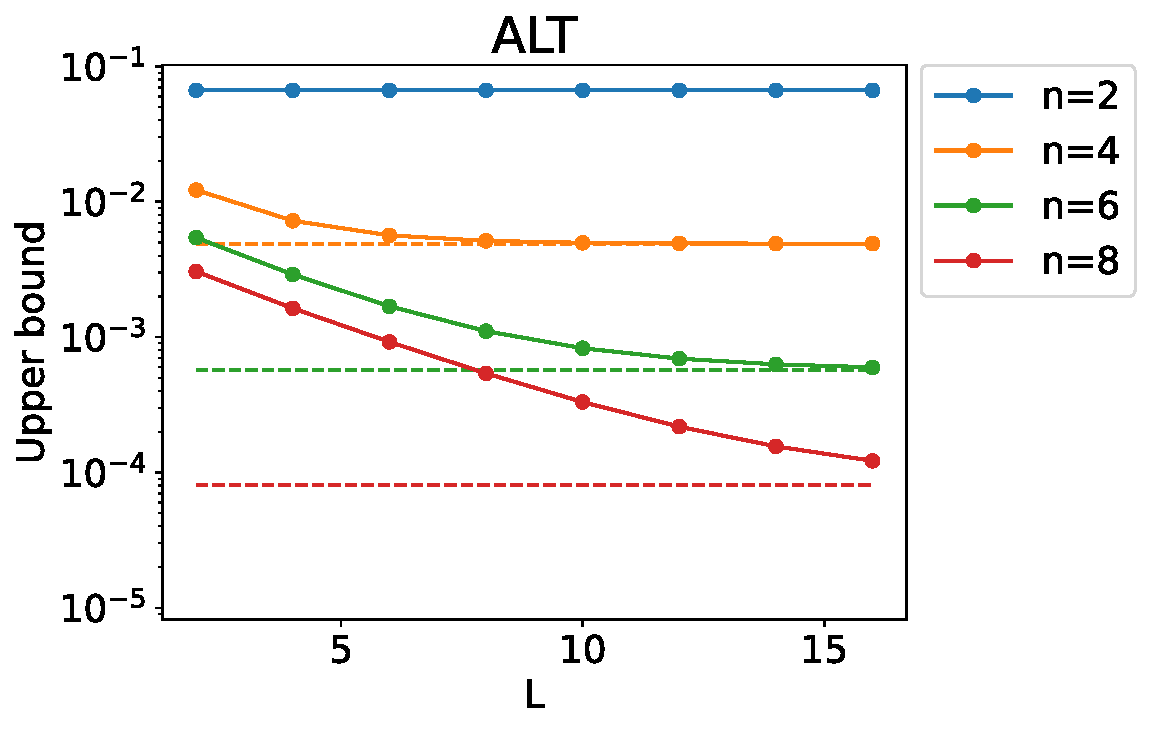
\includegraphics[width=7cm]{qml-var-bound-alt.pdf}
            \end{figure}
        \end{column}
    \end{columns}
    
    \vspace{-10pt}
    \begin{columns}
        \begin{column}{0.5\textwidth}
            \begin{figure}[H]
                \centering
                \begin{tikzpicture}
                    \node[scale=0.6]{
                        \begin{quantikz}
                            \qw & \gate[wires=2,style={fill=cyan!50}][1cm]{}& \qw\\
                            \qw & \qw                  & \qw
                        \end{quantikz}
                        \begin{quantikz}
                            {\LARGE \textbf{=}}
                        \end{quantikz}
                        \begin{quantikz}
                            \qw & \gate{R_x}&\gate{R_y}&\ctrl{1}& \qw\\
                            \qw & \gate{R_x}&\gate{R_y}&\targ{} & \qw
                        \end{quantikz}
                        };
                \end{tikzpicture}
            \end{figure}
            \begin{footnotesize}
                (Define the cost function using the Iris dataset)\\
            \end{footnotesize}
        \end{column}
        \begin{column}{0.5\textwidth}
            \begin{figure}[H]
                \centering
                \begin{tikzpicture}
                    \node[scale=0.6]{
                        \begin{quantikz}
                            \qw & \gate[wires=2,style={fill=cyan!50}][1cm]{}& \qw\\
                            \qw & \qw                  & \qw
                        \end{quantikz}
                        \begin{quantikz}
                            {\LARGE \textbf{=}}
                        \end{quantikz}
                        \begin{quantikz}
                            \text{\LARGE Unitary 2-Design}
                        \end{quantikz}
                        };
                \end{tikzpicture}
            \end{figure}
            \begin{center}
                Indeed, it is an upper bound.
            \end{center}
        \end{column}
    \end{columns}
\end{frame}




\begin{frame}{Necessary Condition for Avoiding Barren Plateau}
    The number of encoding layers for the upper bound not to decay exponentially\\
    \vspace*{10pt}
    \begin{columns}
        \begin{column}{0.65\textwidth}
            \begin{figure}
                \centering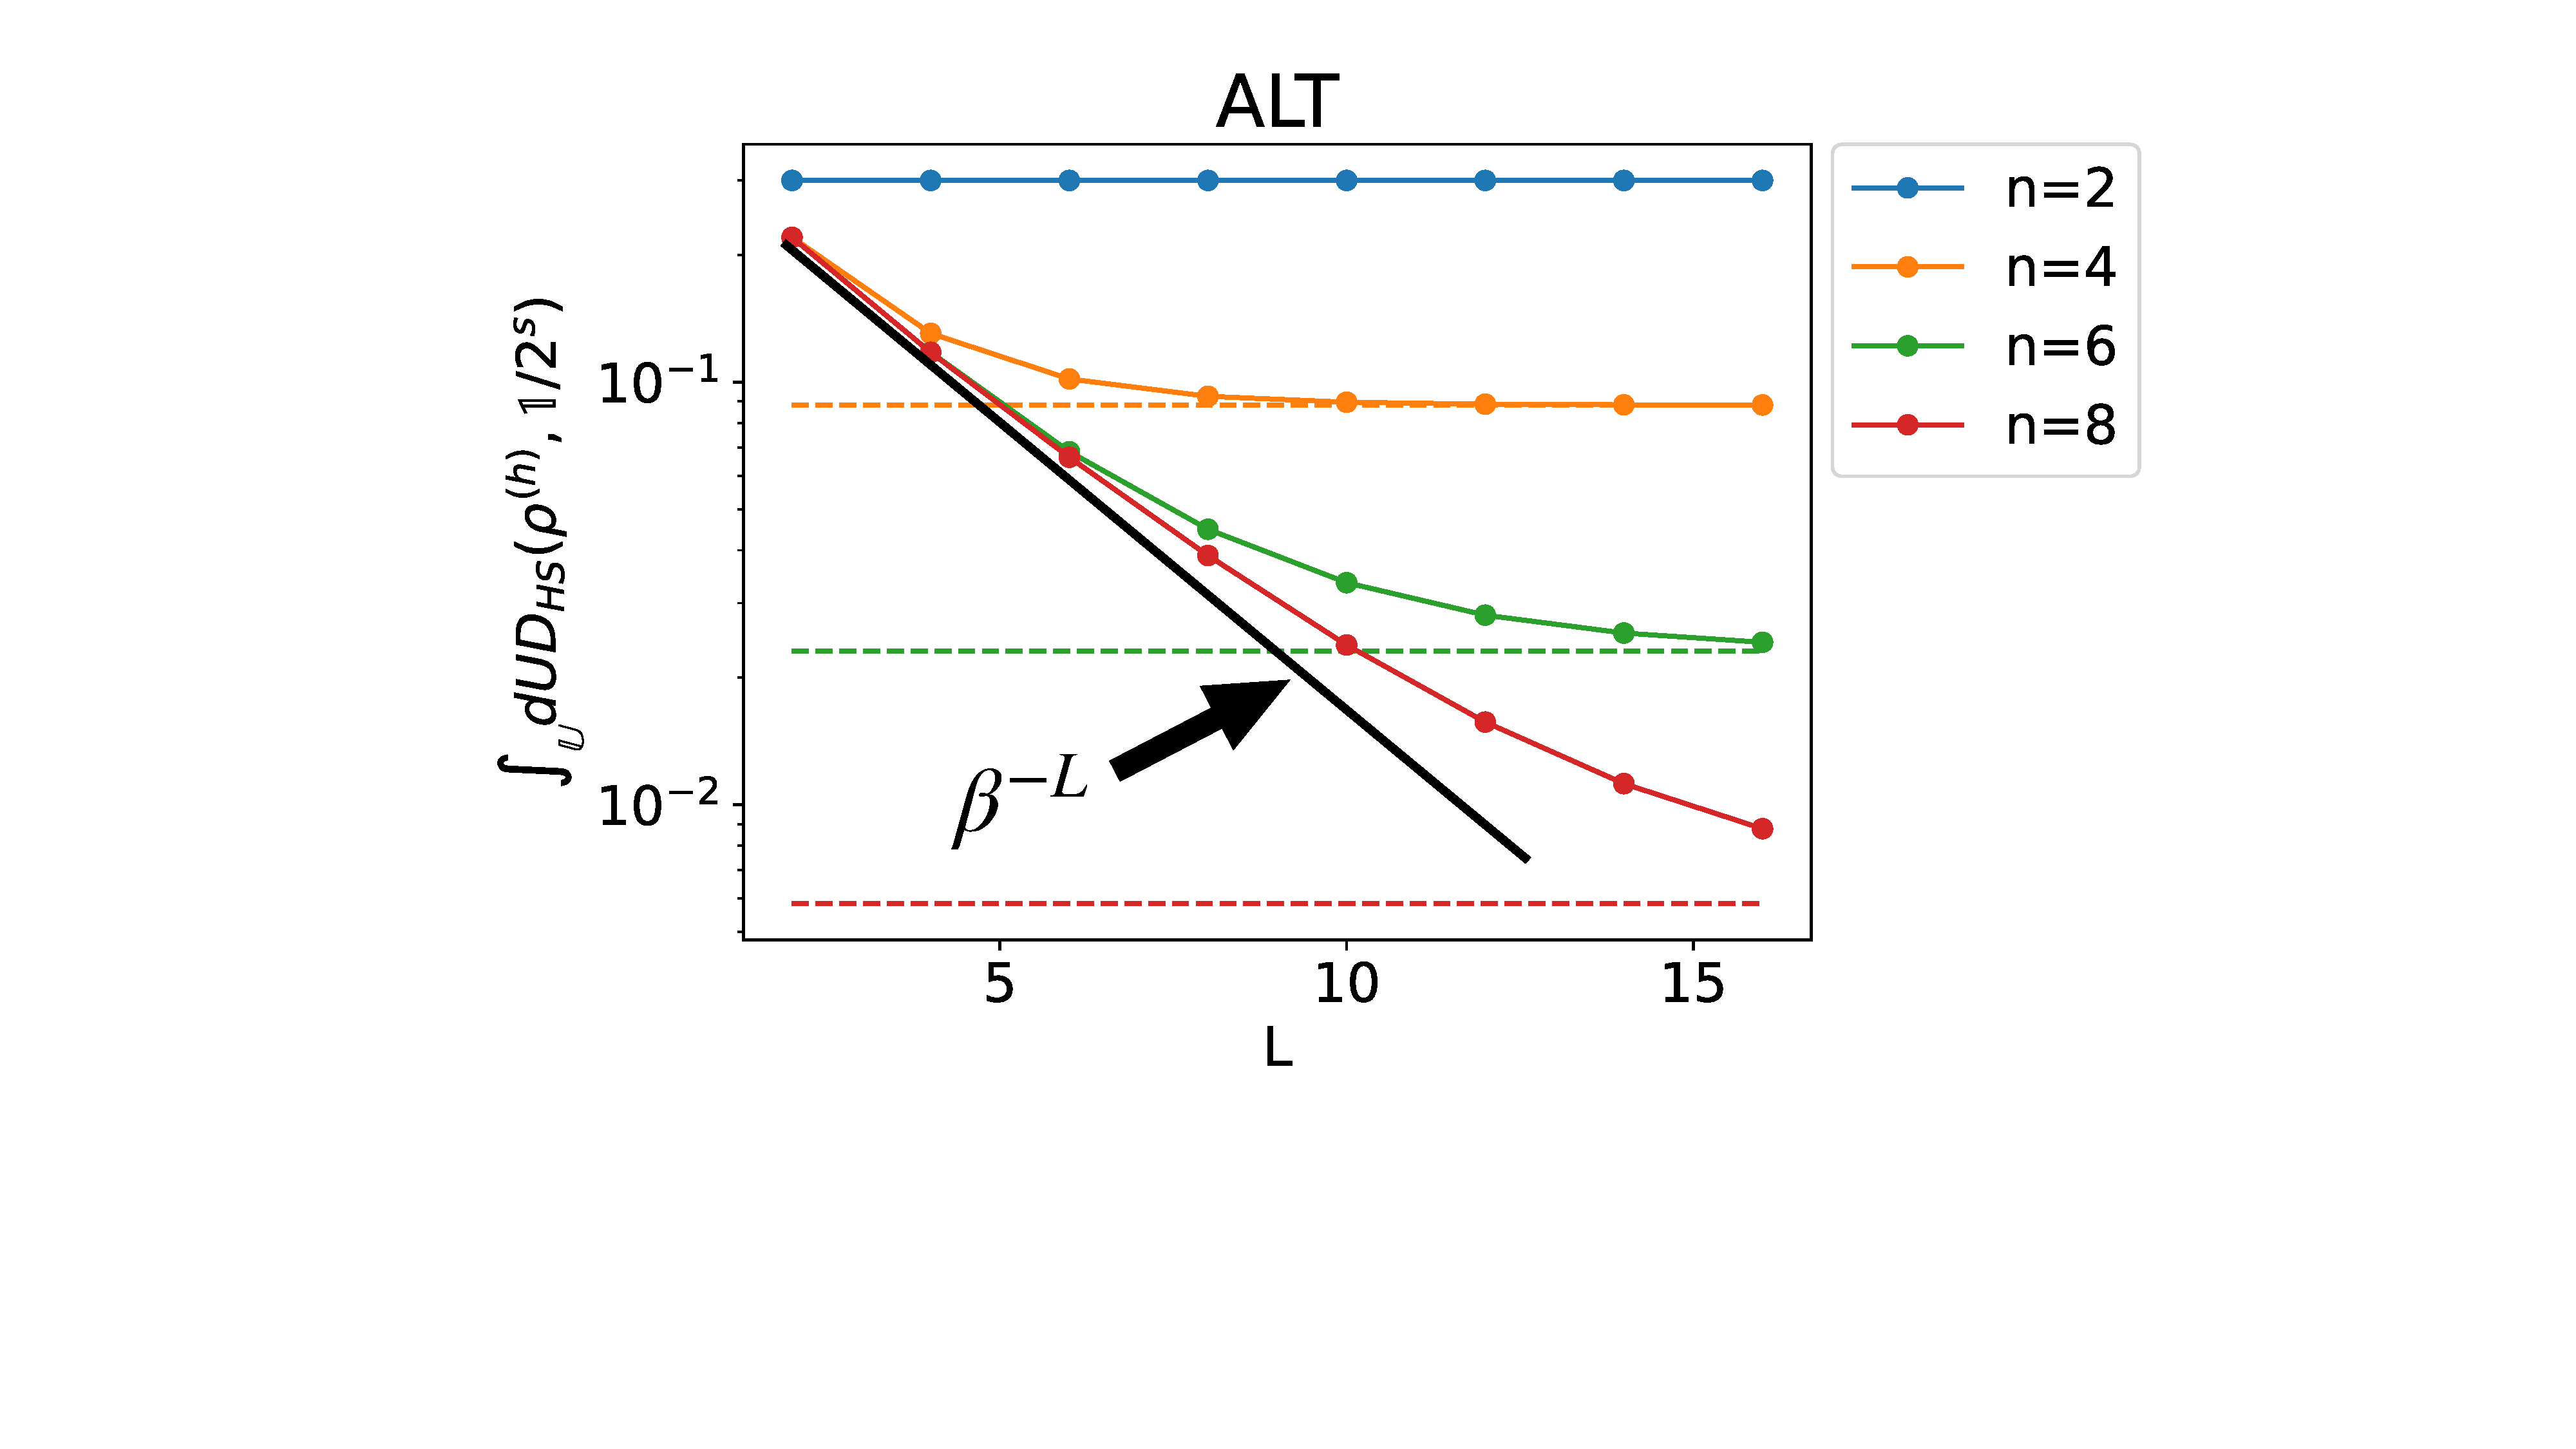
\includegraphics[width=8cm]{hsd-alt-analytical-with-line.pdf}
            \end{figure}
        \end{column}

        \begin{column}{0.35\textwidth}
            {\footnotesize($0<\alpha$, $n$: number of qubits)}\\
            \vspace*{2pt}
            $\bar{D}_{\mathrm{HS}}^s \propto e^{-\alpha n}$\\
            → Barren Plateau\\

            \vspace*{10pt}
            Necessary condition for avoiding Barren Plateau:\\
            {\footnotesize($0<\gamma,\;1<\beta$)}\\
            \vspace*{2pt}
            $n^{-\gamma} \leq \beta^{-L} \leq \bar{D}_{\mathrm{HS}}^s$\\
            \vspace*{2pt}
            \hspace*{5pt}$\;\Longrightarrow\;$ \textcolor{blue}{$L \leq \frac{\gamma}{\log{\beta}}\log{n}$}

        \end{column}
    \end{columns}
\end{frame}





\section{Lower Bound on the Variance of Gradient}
\newcommand{\bgate}[1]{\gate[wires=1,style={fill=cyan!50}][1cm][0.7cm]{\Large #1}}
\newcommand{\rgate}[1]{\gate[wires=4,style={fill=red!50}]{\Large #1}}
\begin{frame}{Lower Bound on the Variance of Gradient: Setup}
    \vspace{-15pt}
    \begin{columns}
        \begin{column}{0.4\textwidth}
            \begin{footnotesize}
                (Simple encoding circuit for analysis)
            \end{footnotesize}
            \begin{itemize}
                \setlength{\itemsep}{5pt}
                \item Quantum circuit: \\$n = s \times \xi$ qubits\\Encoding consists of $R_y$
                \item Cost function ($y_i\in \{0,1\}$): $\calL_{\mathrm{MAE}}(\bth) = \frac1N\sum_{i=1}^N |\ell_{i}(\bth) - y_i|$
                \item Input data: \\$\calX = \{\bs{x}\}$ (label $0$)\\$\calZ = \{\bs{z}\}$ (label $1$)\\$|\calX|:|\calZ| = p:q\;(p+q=1)$
                \item Gaussian distribution: $x_{j,d} \sim \calN(\mu_{x|j,d}, \sigma_{x|j,d}^2)$\\$z_{j,d} \sim \calN(\mu_{z|j,d}, \sigma_{z|j,d}^2)$
                \item Variance: $\sigma_{x|j,d},\, \sigma_{z|j,d} \leq \sigma_{\max}$
            \end{itemize}
        \end{column}
        \begin{column}{0.5\textwidth}
        \begin{figure}[H]
            \centering
            \begin{tikzpicture}
            \node[scale=0.45]{
                \begin{quantikz}
                    \lstick{$\ket{0}$} & \bgate{R_y(x_{1,1})}    & \bgate{R_y(x_{1,2})}    &\qw \ \ldots\ & \bgate{R_y(x_{1,L})}    &\rgate{V_1(\bth_1)}& \meter{} \\
                    \lstick{$\ket{0}$} & \bgate{R_y(x_{2,1})}    & \bgate{R_y(x_{2,2})}    &\qw \ \ldots\ & \bgate{R_y(x_{2,L})}    & \qw                     & \meter{} \\
                    \wave&&&&&&&&&\\
                    \lstick{$\ket{0}$} & \bgate{R_y(x_{s,1})}    & \bgate{R_y(x_{s,2})}    &\qw \ \ldots\ & \bgate{R_y(x_{s,L})}    & \qw                     & \meter{}\\
                    \lstick{$\ket{0}$} & \bgate{R_y(x_{s+1,1})}  & \bgate{R_y(x_{s+1,2})}  &\qw \ \ldots\ & \bgate{R_y(x_{s+1,L})}  &\rgate{V_2(\bth_2)}& \meter{} \\
                    \lstick{$\ket{0}$} & \bgate{R_y(x_{s+2,1})}  & \bgate{R_y(x_{s+2,2})}  &\qw \ \ldots\ & \bgate{R_y(x_{s+2,L})}  & \qw                     & \meter{} \\
                    \wave&&&&&&&&&\\
                    \lstick{$\ket{0}$} & \bgate{R_y(x_{2s,1})}   & \bgate{R_y(x_{2s,2})}   &\qw \ \ldots\ & \bgate{R_y(x_{2s,L})}   & \qw                     & \meter{}\\
                    \wave&&&&&&&&&\\
                    \lstick{$\ket{0}$} & \bgate{R_y(x_{n-s+1,1})}& \bgate{R_y(x_{n-s+1,2})}&\qw \ \ldots\ & \bgate{R_y(x_{n-s+1,L})}&\rgate{V_\xi(\bth_\xi)}& \meter{} \\
                    \lstick{$\ket{0}$} & \bgate{R_y(x_{n-s+2,1})}& \bgate{R_y(x_{n-s+2,2})}&\qw \ \ldots\ & \bgate{R_y(x_{n-s+2,L})}& \qw                     & \meter{} \\
                    \wave&&&&&&&&&\\
                    \lstick{$\ket{0}$} & \bgate{R_y(x_{n,1})}    & \bgate{R_y(x_{n,2})}    &\qw \ \ldots\ & \bgate{R_y(x_{n,L})}    & \qw                     & \meter{}
                \end{quantikz}};
            \end{tikzpicture}
            \caption{$L$ layers of $R_y$ gates encoding circuit and\\$\xi$ $s$-qubit unitaries $V_\xi(\bth_\xi)$ for the ansatz}
            \label{fig:circuit-concentration-1}
        \end{figure}
        \end{column}
    \end{columns}
\end{frame}



\begin{frame}{Lower Bound on the Variance of Gradient: Results}
    \begin{theorem}
        Lower bound on the variance of the cost function gradient is given as follows,
        \begin{align*}
            \frac{r_{n,s}}{2^s}\;
            \sum_{j=1}^s \qty(p\,e^{-\Sigma_{x|j}/2} - q\,e^{-\Sigma_{z|j}/2})^2
            \leq \Var_{V(\bth)}[\pd_\nu\calL_{\mathrm{MAE}}(\bth)]
        \end{align*}
        where $r_{n,s} := \frac{s\,2^{3(s-1)}}{n^2(2^{2s}-1)^2}$, $\Sigma_{x|j} = \sum_{d=1}^L \sigma_{x|j,d}^2$, $\Sigma_{z|j} = \sum_{d=1}^L \sigma_{z|j,d}^2$
    \end{theorem}
    
    For $|\calX|:|\calZ| = 1:1 \iff p = q = 1/2$, the lower bound is
    \begin{center}
        $
        \frac{r_{n,s}}{2^{s+2}}\;
        \sum_{j=1}^s
        \qty(e^{-\Sigma_{x|j}/2}- e^{-\Sigma_{z|j}/2})^2
        \leq \Var_{V(\bth)}[\pd_\nu\calL_{\mathrm{MAE}}(\bth)]
        $
    \end{center}

    \begin{itemize}
        \item The difference between $e^{-\Sigma_{x|j}/2}$ and $e^{-\Sigma_{z|j}/2}$ is crucial in the lower bound
        \item However, $e^{-\Sigma_{x|j}/2}$ and $e^{-\Sigma_{z|j}/2}$ decay exponentially with \#(encoding layers)
        \item If $e^{-\Sigma_{x|j}/2} = e^{-\Sigma_{z|j}/2}$ for all $j$, the lower bound becomes $0$
    \end{itemize}
\end{frame}




\begin{frame}{Lower Bound on the Variance of Gradient: Results}
    \begin{theorem}
        Lower bound on the variance of the cost function gradient is given as follows,
        \begin{align*}
            \frac{r_{n,s}}{2^s}\;
            \sum_{j=1}^s \qty(p\,e^{-\Sigma_{x|j}/2} - q\,e^{-\Sigma_{z|j}/2})^2
            \leq \Var_{V(\bth)}[\pd_\nu\calL_{\mathrm{MAE}}(\bth)]
        \end{align*}
        where $r_{n,s} := \frac{s\,2^{3(s-1)}}{n^2(2^{2s}-1)^2}$, $\Sigma_{x|j} = \sum_{d=1}^L \sigma_{x|j,d}^2$, $\Sigma_{z|j} = \sum_{d=1}^L \sigma_{z|j,d}^2$
    \end{theorem}
    
    For $|\calX|:|\calZ| = 1:0 \iff p = 1,\,q = 0$, the lower bound is
    \begin{center}
        $
            \frac{r_{n,s}s}{2^s}\; e^{-L\sigma_{\max}^2}
            \leq \frac{r_{n,s}}{2^s}\;\sum_{j=1}^s e^{-\Sigma_{x|j}}
            \leq \Var_{V(\bth)}[\pd_{\theta_\nu}\calL_{\mathrm{MAE}}(\bth)]
        $
    \end{center}

    \begin{itemize}
        \item Large lower bound when $L\sigma_{\max}^2$ is small
        \item If $s, L\sigma_{\max}^2 \in \mathcal{O}(\log{n})$, the lower bound becomes $\mathcal{O}(1/\text{poly}(n))$\\ → Sufficient condition for avoiding barren plateaus
    \end{itemize}
\end{frame}



\section{Form of Function $f$ and Variance of Gradient}
\begin{frame}{Form of Function $f$ and Variance of Gradient}
    How does the function $f$ affect the scaling of variance of gradient?
    \begin{footnotesize}
        \begin{align*}
            \calL_{\mathrm{MAE}}(\bth) &= \frac1N\sum_{i=1}^N \abs{\ell_i(\bth) - y_i} \\
            \calL_{\mathrm{MSE}}(\bth) &= \frac1N\sum_{i=1}^N \qty(\ell_i(\bth) - y_i)^2 \\
            \calL_{\mathrm{LOG}}(\bth) &= \frac1N\sum_{i=1}^N [-y_i \log{\ell_i(\bth)} - (1-y_i)\log{(1-\ell_i(\bth))}] \\
        \end{align*}
        \vspace{-25pt}
        \begin{alignat*}{2}
            \implies
            \pd_{\theta_\nu} \calL_{\mathrm{MAE}}(\bth) &= \frac1N\sum_{i=1}^N &\sgn(\ell_i(\bth) - y_i) \cdot\pd_{\theta_\nu} \ell_i(\bth) \\
            \pd_{\theta_\nu} \calL_{\mathrm{MSE}}(\bth) &= \frac1N\sum_{i=1}^N 2|\ell_i(\bth) - y_i| &\sgn(\ell_i(\bth) - y_i)\cdot\pd_{\theta_\nu} \ell_i(\bth) \\
            \pd_{\theta_\nu} \calL_{\mathrm{LOG}}(\bth) &= \frac1N\sum_{i=1}^N \frac{1}{1 - |\ell_i(\bth) - y_i|} &\sgn(\ell_i(\bth) - y_i) \cdot\pd_{\theta_\nu} \ell_i(\bth) 
        \end{alignat*}
    \end{footnotesize}
    \begin{center}
        where $y_i \in \{0,1\}$, $\quad \ell_i(\bth) = \Tr[\rho_i(\bth)\,O_L] \in [0,1]$,   $\quad (O_L = \frac1n \sum_{j=1}^{n}\dyad{0}_{j} \otimes \bbid_{\bar{j}})$
    \end{center}
\end{frame}




\begin{frame}{Form of Function $f$ and Variance of Gradient}
    Assuming the ansatz is a unitary $2$-design, the mean and variance of $\ell_i(\bth)$ are:
    \begin{align*}
        \E_{\calU(d)}[\ell_i(\bth)]  &= \frac12\\
        \Var_{\calU(d)}[\ell_i(\bth)]&= \frac{1}{4n(2^n+1)}
    \end{align*}
    Therefore, assuming $\ell_i(\bth) \sim \frac12$ for all $i$ $\iff |\ell_i(\bth) - y_i| \sim \frac12$ we get:
    \begin{align*}
        \pd_{\theta_\nu} \calL_{\mathrm{MSE}}(\bth) \sim \pd_{\theta_\nu} \calL_{\mathrm{MAE}}(\bth),\quad
        \pd_{\theta_\nu} \calL_{\mathrm{LOG}}(\bth) \sim 2\,\pd_{\theta_\nu} \calL_{\mathrm{MAE}}(\bth)
    \end{align*}
    Thus, the ratio of the variance of the gradients for mean squared error to mean absolute error, and cross-entropy error to mean absolute error, is approximately:
    \begin{align*}
        \implies
        \frac{\Var_{\calU(d)}[\pd_{\theta_\nu}\calL_{\mathrm{MSE}}(\bth)]}{\Var_{\calU(d)}[\pd_{\theta_\nu}\calL_{\mathrm{MAE}}(\bth)]} &\sim 1\\
        \frac{\Var_{\calU(d)}[\pd_{\theta_\nu}\calL_{\mathrm{LOG}}(\bth)]}{\Var_{\calU(d)}[\pd_{\theta_\nu}\calL_{\mathrm{MAE}}(\bth)]} &\sim 4
    \end{align*}
    When the ansatz is deep, the scaling of the variance of gradient seems to be similar regardless of the function $f$.
\end{frame}



\newcommand{\rgbt}{\gate[wires=2,style={fill=red!50}][1cm][0.1cm]{}}
\newcommand{\bgbo}{\gate[wires=1,style={fill=cyan!50}][1cm][0.5cm]{}}
\newcommand{\bgbog}{\gate[wires=1,style={fill=cyan!50}][1cm][0.5cm]{}\gategroup[wires=8,steps=4,style={dashed, rounded corners, fill=cyan!20, inner xsep=1pt},background,label style={label position=below,anchor=north,yshift=-0.2cm}]{{\Large Shallow}}}
\newcommand{\gpd}{\ghost{H}\gategroup[wires=8,steps=11,style={dashed, rounded corners, fill=red!20, inner xsep=3pt, inner ysep=21pt},background,label style={label position=below,anchor=north,yshift=-0.2cm}]{{\Large Deep}}}
\begin{frame}{Form of Function $f$ and Variance of Gradient}
    Assuming ALT for the ansatz, we examine the ratio of variance of the cost function gradient when the number of layers $L_{\text{red}}$ is varied. (Blue represents the encoding circuit, red represents the ansatz.)
    \begin{figure}[H]
        \centering
        \begin{tikzpicture}
            \node[scale=0.6]{
            \begin{quantikz}
                \gpd     & \bgbog& \bgbo & \bgbo &\rgbt & \qw  &\rgbt & \qw  &\qw\ \ldots\ &\rgbt & \qw\\[-0.3cm]
                \ghost{H}& \bgbo & \bgbo & \bgbo & \qw  & \rgbt& \qw  & \rgbt&\qw\ \ldots\ & \qw  & \qw\\[-0.3cm]
                \ghost{H}& \bgbo & \bgbo & \bgbo & \rgbt& \qw  & \rgbt& \qw  &\qw\ \ldots\ & \rgbt& \qw\\[-0.3cm]
                \ghost{H}& \bgbo & \bgbo & \bgbo & \qw  & \rgbt& \qw  & \rgbt&\qw\ \ldots\ & \qw  & \qw\\[-0.3cm]
                \ghost{H}& \bgbo & \bgbo & \bgbo & \rgbt& \qw  & \rgbt& \qw  &\qw\ \ldots\ & \rgbt& \qw\\[-0.3cm]
                \ghost{H}& \bgbo & \bgbo & \bgbo & \qw  & \rgbt& \qw  & \rgbt&\qw\ \ldots\ & \qw  & \qw\\[-0.3cm]
                \ghost{H}& \bgbo & \bgbo & \bgbo & \rgbt& \qw  & \rgbt& \qw  &\qw\ \ldots\ & \rgbt& \qw\\[-0.3cm]
                \ghost{H}& \bgbo & \bgbo & \bgbo & \qw  & \qw  & \qw  & \qw  &\qw\ \ldots\ & \qw  & \qw
            \end{quantikz}
            };
        \end{tikzpicture}
    \end{figure}
    
    \vspace{-27pt}
    \begin{columns}
        \begin{column}{0.5\textwidth}
            \begin{figure}[H]
                \centering
                \begin{tikzpicture}
                    \node[scale=0.8]{
                        \begin{quantikz}
                            \qw & \gate[wires=1,style={fill=cyan!50}][1cm][0.7cm]{}& \qw
                        \end{quantikz}
                        \begin{quantikz}
                            {\LARGE \textbf{=}}
                        \end{quantikz}
                        \begin{quantikz}
                            \qw & \gate{R_x} &\gate{R_y} & \qw
                        \end{quantikz}
                        };
                \end{tikzpicture}
            \end{figure}
        \end{column}
        
        \begin{column}{0.5\textwidth}
            \begin{figure}[H]
                \centering
                \begin{tikzpicture}
                    \node[scale=0.7]{
                        \begin{quantikz}
                            \qw & \gate[wires=2,style={fill=red!50}][1cm]{}& \qw\\
                            \qw & \qw                  & \qw
                        \end{quantikz}
                        \begin{quantikz}
                            {\LARGE \textbf{=}}
                        \end{quantikz}
                        \begin{quantikz}
                            \qw & \gate{R_x}&\gate{R_y}&\ctrl{1}& \qw\\
                            \qw & \gate{R_x}&\gate{R_y}&\targ{} & \qw
                        \end{quantikz}
                        };
                \end{tikzpicture}
            \end{figure}
        \end{column}
    \end{columns}
\end{frame}




\begin{frame}{Form of Function $f$ and Variance of Gradient}
    \vspace{-10pt}
    \begin{columns}
        \begin{column}{0.5\textwidth}
            \begin{figure}
                \centering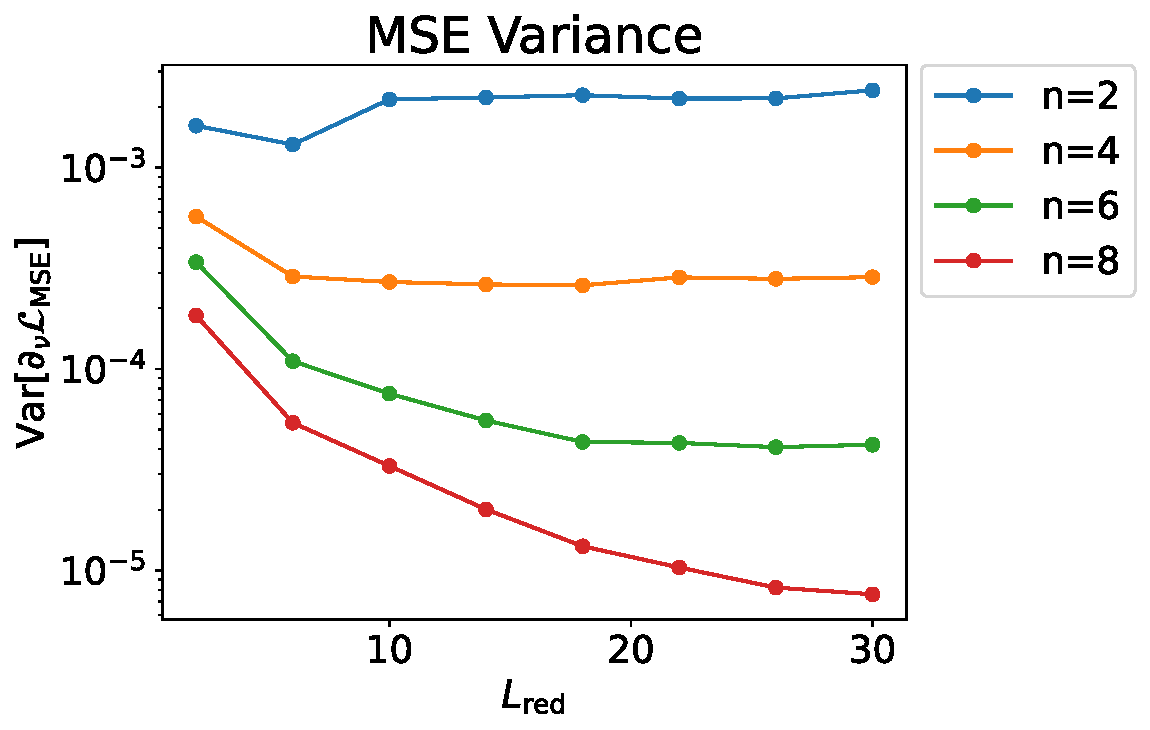
\includegraphics[width=6cm]{variance-mse_encoding3.pdf}
            \end{figure}
        \end{column}
        \begin{column}{0.5\textwidth}
            \begin{figure}
                \centering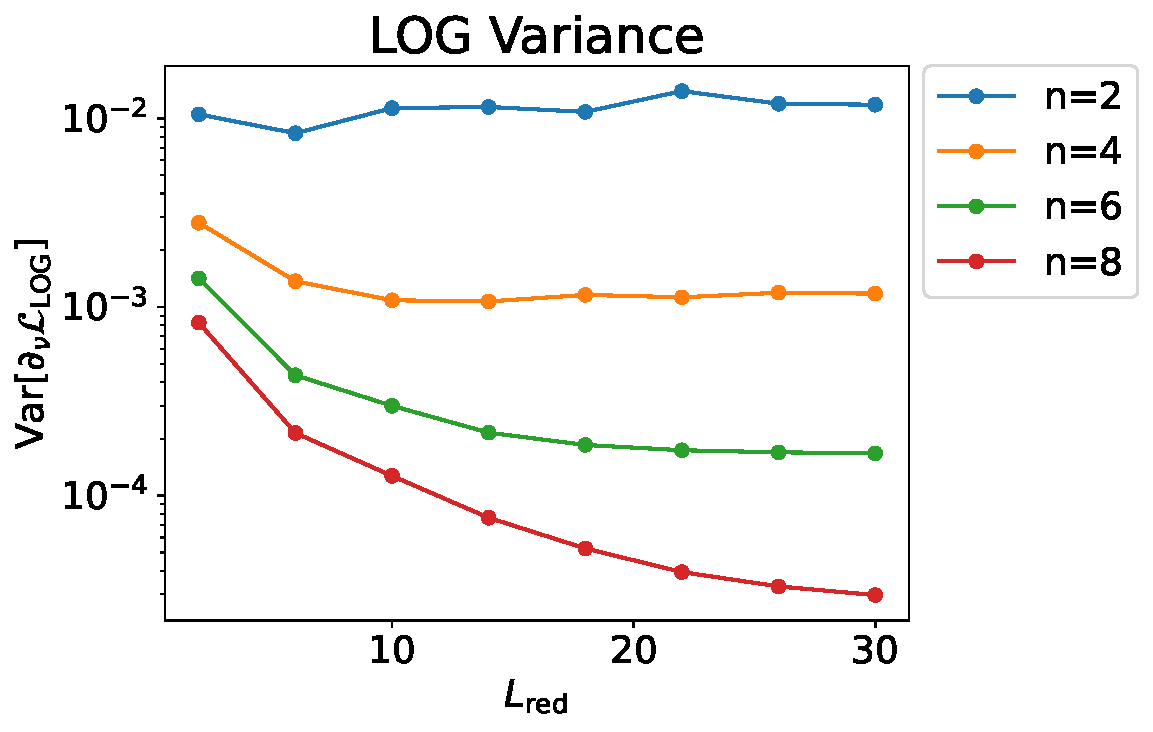
\includegraphics[width=6cm]{variance-log_encoding3.pdf}
            \end{figure}
        \end{column}
    \end{columns}
    \vspace{-15pt}
    \begin{figure}
        \centering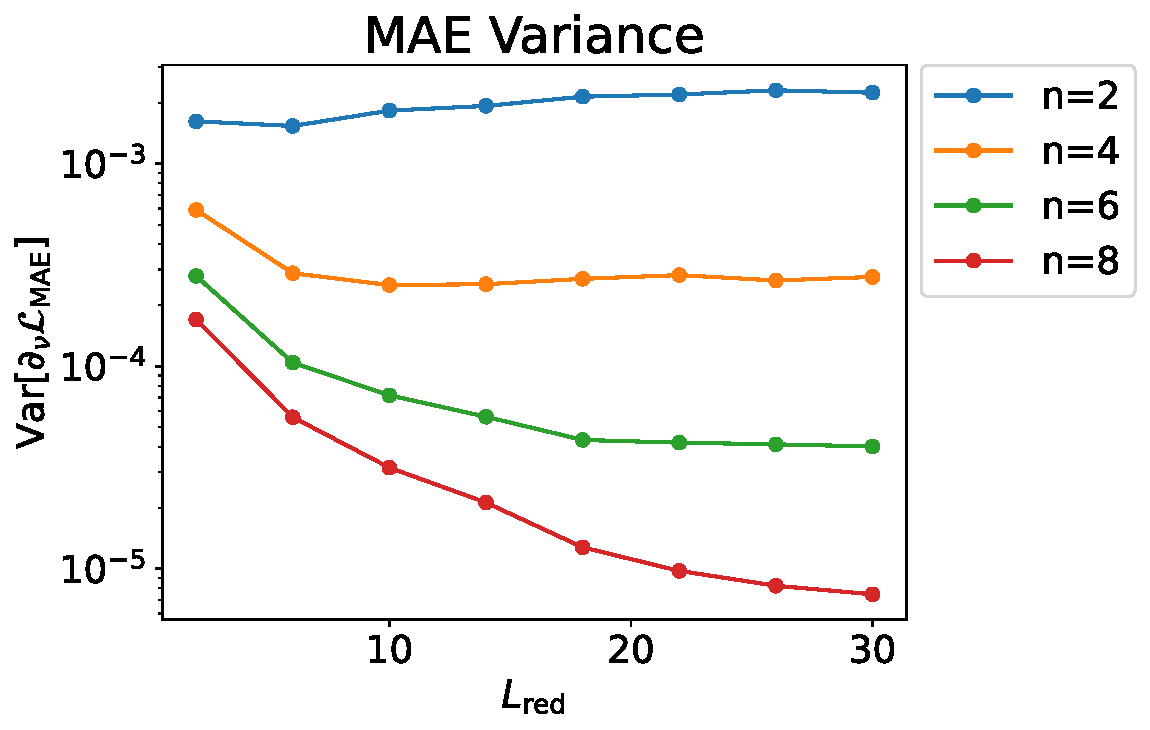
\includegraphics[width=6cm]{variance-mae_encoding3.pdf}
    \end{figure}
\end{frame}




\begin{frame}{Form of Function $f$ and Variance of Gradient}
    \begin{columns}
        \begin{column}{0.5\textwidth}
            \begin{small}
                \centering\hspace*{-10pt} $\Var_{V(\bth)}[\pd_{\theta_\nu}\calL_{\mathrm{MSE}}(\bth)]\,/\,\Var_{V(\bth)}[\pd_{\theta_\nu}\calL_{\mathrm{MAE}}(\bth)]$
            \end{small}
            \begin{figure}
                \centering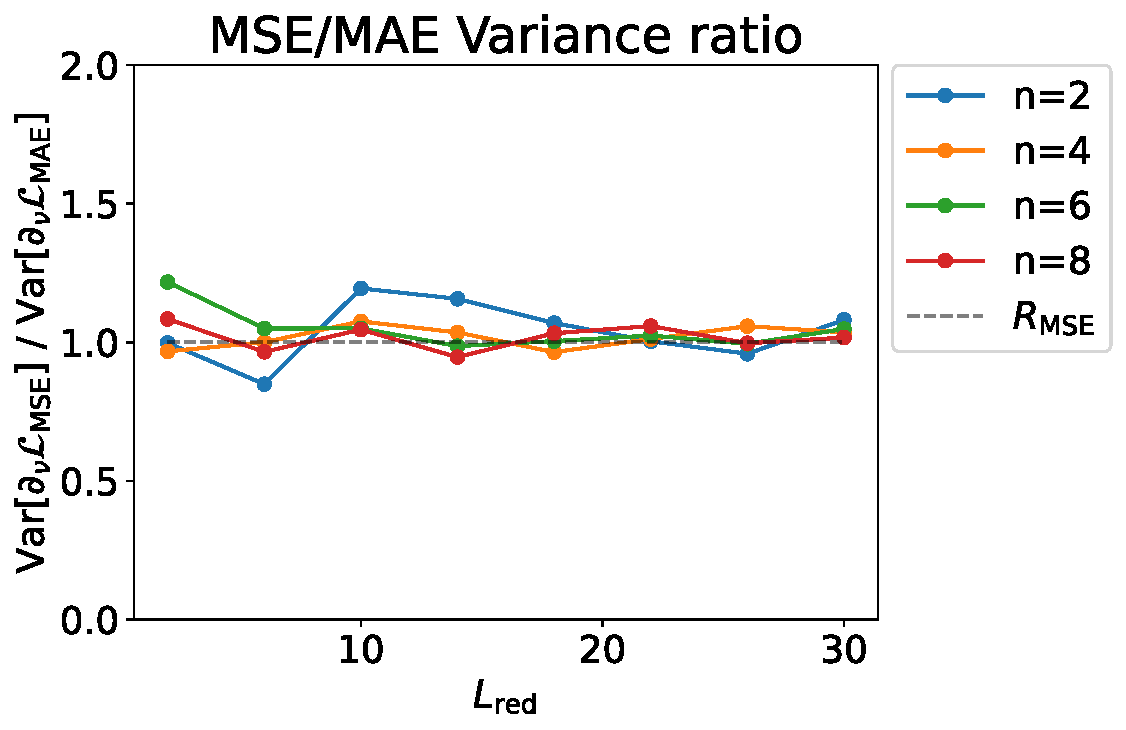
\includegraphics[width=7cm]{variance-mse-mae-ratio_encoding3.pdf}
                \caption{Dashed line is the approximation ratio $R_{\mathrm{MSE}}=1$}
            \end{figure}
        \end{column}
        \begin{column}{0.5\textwidth}
            \begin{small}
                \centering\hspace*{-10pt} $\Var_{V(\bth)}[\pd_{\theta_\nu}\calL_{\mathrm{LOG}}(\bth)]\,/\,\Var_{V(\bth)}[\pd_{\theta_\nu}\calL_{\mathrm{MAE}}(\bth)]$
            \end{small}
            \begin{figure}
                \centering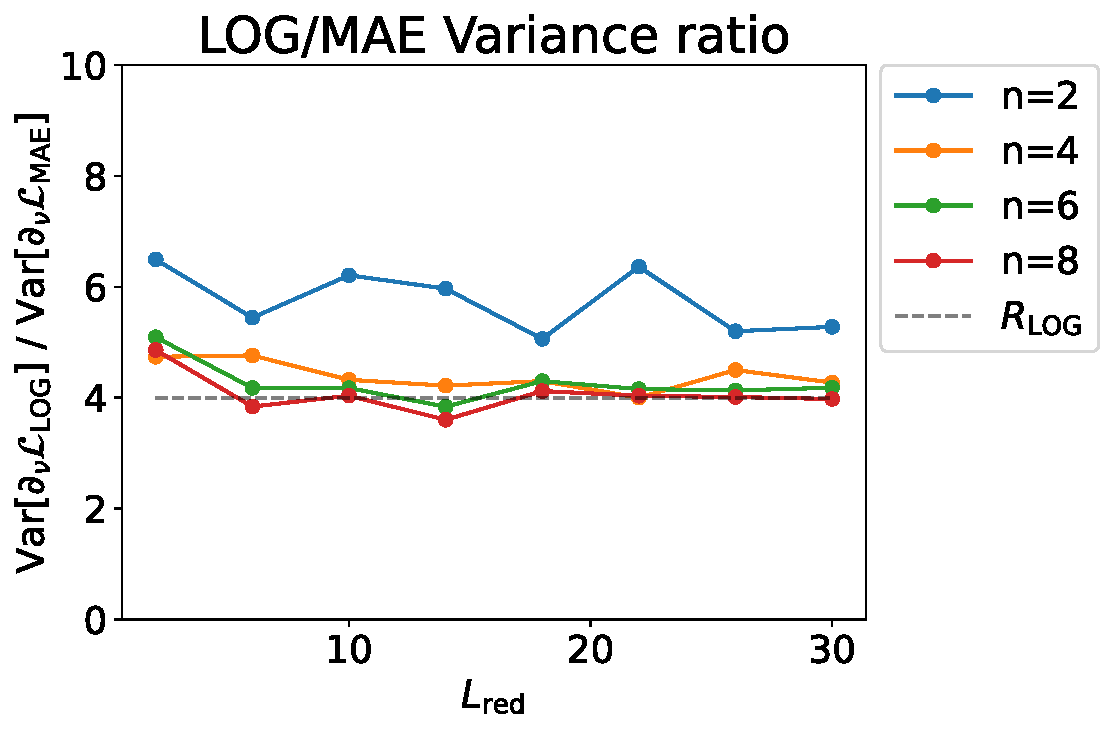
\includegraphics[width=7cm]{variance-log-mae-ratio_encoding3.pdf}
                \caption{Dashed line is the approximation ratio $R_{\mathrm{LOG}}=4$}
            \end{figure}
        \end{column}
    \end{columns}
    \centering
    \hspace{-10pt}In numerical calculations, the scaling of the variance of gradient seems to be similar regardless of the function $f$, even for shallow circuits.\\
    
    \begin{scriptsize}
        (Cost functions were defined using the Iris dataset.)
    \end{scriptsize}
\end{frame}



\section{Summary}
\begin{frame}{Summary and Future Work}
    \vspace*{-15pt}
    \hspace*{-50pt}

    \begin{center}
        {\large\colorbox{blue!40}{\makebox[27em]{Study on the Influence of Data Encoding on Barren Plateaus}}}
    \end{center}

    \begin{itemize}
        \item Derived and numerically validated an upper bound on variance of the gradient from the perspective of data encoding
        \item Increased entanglement in the state after data encoding and expressive power of the encoding circuit lead to a smaller upper bound, resulting in barren plateau.
        \item If \#layers for data encoding is $O(\log{n})$, the upper bound won't decay exponentially.
        \item For input data following a Gaussian distribution, the data variance is crucial for the lower bound on the variance of gradient
        \item Numerically confirmed that the scaling of the variance of gradient is almost independent of the form of the function $f$
    \end{itemize}

    \begin{center}
        {\large\colorbox{blue!40}{\makebox[15em]{Future Work}}}
    \end{center}

    \begin{itemize}
        \item Investigate the lower bound for more general encoding circuits.
        \item Consider encoding eircuits from the perspective of generalization performance.
        \item Examine whether the encoding circuit is classically hard to simulate.
    \end{itemize}
    % Once the scaling is understood, it can be used to estimate the potential lower bounds on computational complexity for a given setting.
\end{frame}



\appendix
\begin{frame}{On the Locality of Observables}
    Local observable
    \begin{itemize}
        \item $Z_1 := Z \ot \bbid \ot \bbid \ot \cdots \ot \bbid$
        \item $\dyad{0}_1 = (Z_1 + \bbid_1)/2$
        \item $O_L := \frac1n \sum_{j=1}^{n}\dyad{0}_{j} \otimes \bbid_{\bar{j}}$ (linear combination of local observables)
        \item If the depth of ALT ansatz is $\order{\log{n}}$, no barren plateau (without data encoding)
    \end{itemize}
    
    Global observable
    \begin{itemize}
        \item $Z\otn{n} := Z \ot Z \ot \cdots \ot Z$
        \item The barren plateau occurs regardless of the depth of the ansatz.
    \end{itemize}
\end{frame}



\begin{frame}{Unitary $t$--design}
    \begin{definition}
        Let $P_{t,t}(U)$ be a homogeneous polynomial of maximum degree $t$ in the components of the unitary $U$ and $U\dg$. A set of $K$ unitaries $\{U_k\}$ is said to be a unitary $t$--design if it satisfies the following condition. (ex. $P_{2,2}(U) = U\dg AUBU\dg CU$)
        \begin{align*}
            \frac1K \sum_{k=1}^{K} P_{t}(U_k) = \int_{\calU(d)}P_{t} (U) d\mu(U)
        \end{align*}
    \end{definition}
    
    \begin{itemize}
        \item Pauli group: $\mathcal{P}(n)=\{e^{i\frac{k\pi}{2}}\, P_{j_1}\otimes \cdots\otimes P_{j_n}| k,j_l=0,1,2,3\}$ is a unitary $1$--design
        \item Clifford group: $\mathcal{C}(n)=\{U\in \mathcal{U}(2^n)|\,UPU^\dagger = \mathcal{P}(n)\}$ is a unitary $3$--design
        \item If $\{U_k\}$ is a unitary $t$--design, it is also a unitary $(t-1)$--design.
    \end{itemize}
\end{frame}




\begin{frame}{Avoiding Barren Plateaus}
    \begin{itemize}
        \item (Without data encoding) It has been shown that the barren plateau does not occur if the depth of the ansatz is $\order{\log{n}}$ when using local observables. %\cite{cerezo2021cost}
        \item Optimize the parameters for each layer of the ansatz. This reduces the effective depth of the ansatz. %\cite{skolik2021layerwise}
        \item Set the initial values of some of the parameters to cancel out the rest of the circuit. This reduces the effective depth of the ansatz. %\cite{grant2019initialization}
        \item Introduce correlations between parameters. This reduces the expressibility of the ansatz. %\cite{holmes2022connecting}
        \item Sample the initial values of the parameters from a normal distribution instead of a uniform distribution. %\cite{zhang2022escaping}
    \end{itemize}
\end{frame}



\definecolor{circleColor}{RGB}{100,180,44}   % Green
\definecolor{ellipseColor}{RGB}{65,160,241}  % Blue
\begin{frame}{Expressibility}
    The expressibility of a quantum circuit is defined as follows.
    \begin{align*}
        \epsilon_{\bbU}^{(t,p)}(X) &:= \norm{A^{(t)}_{\bbU}(X)}_p,\\
        \calA_{\bbU}^{(t)}(X) &:= \int_{{\color{circleColor} \calU(d)}} d\mu_{\Haar}(V)\,V\otn{t}X\otn{t}(V\otn{t})\dg - \int_{{\color{ellipseColor} \bbU}} dU\,U\otn{t}X\otn{t}(U\otn{t})\dg.
    \end{align*}

    \begin{columns}
        \hspace*{40pt}
        \begin{column}{0.5\textwidth}
            \begin{itemize}
                \item $\norm{\cdot}_p$:Schatten $p$--norm
                \item $X$:Initial state $\dyad{0}^{\otimes n}$
                \item $\calU(d)$:Unitary group of dimension $d$
                \item Consider the case of $t=2$
            \end{itemize}
        \end{column}

        \begin{column}{0.5\textwidth}
            \begin{figure}[H]
                \centering
                \begin{tikzpicture}[scale=0.5]
                    \definecolor{circleColor}{RGB}{100,180,44}   % Green
                    \definecolor{ellipseColor}{RGB}{65,160,241}  % Blue
                    % Draw the circle
                    \draw[fill=circleColor, draw=black] (0,0) circle (3.2cm);
                    % Add text inside the circle
                    \node at (0,1.5) {\small Unitary group $\calU(d)$};
                  
                    % Draw the ellipse inside the circle
                    \draw[fill=ellipseColor, draw=black] (-0.5,-0.9) ellipse (2.5cm and 1.5cm);
                    % Add text inside the ellipse
                    \node at (-0.5,-0.9) {\small Accesible set $\bbU$};
                    \end{tikzpicture}
                \caption{Expressible region of a quantum circuit}
            \end{figure}
        \end{column}
    \end{columns}
\end{frame}



\begin{frame}{Expressibility: Circuit}
    \begin{columns}
        \begin{column}{0.5\textwidth}
            \centering\hspace*{-30pt} Tensor Product Ansatz
            \begin{tikzpicture}
                \node[scale=0.55]{
                \begin{quantikz}
                    \lstick{$\ket{0}$}\slice{} & \gate{R_x} & \gate{R_y}\slice{1}& \gate{R_x} & \gate{R_y}\slice{2}& \gate{R_x} & \gate{R_y}\slice{3}& \meter{}\\
                    \lstick{$\ket{0}$}      & \gate{R_x} & \gate{R_y}      & \gate{R_x} & \gate{R_y}      & \gate{R_x} & \gate{R_y}      & \meter{}\\
                    \lstick{$\ket{0}$}      & \gate{R_x} & \gate{R_y}      & \gate{R_x} & \gate{R_y}      & \gate{R_x} & \gate{R_y}      & \meter{}\\
                    \lstick{$\ket{0}$}      & \gate{R_x} & \gate{R_y}      & \gate{R_x} & \gate{R_y}      & \gate{R_x} & \gate{R_y}      & \meter{}\\
                    \lstick{$\ket{0}$}      & \gate{R_x} & \gate{R_y}      & \gate{R_x} & \gate{R_y}      & \gate{R_x} & \gate{R_y}      & \meter{}\\
                    \lstick{$\ket{0}$}      & \gate{R_x} & \gate{R_y}      & \gate{R_x} & \gate{R_y}      & \gate{R_x} & \gate{R_y}      & \meter{}
                \end{quantikz}
                };
            \end{tikzpicture}
        \end{column}
        
        \begin{column}{0.5\textwidth}
            \centering\hspace*{-30pt} Alternating Layered Ansatz
            \begin{tikzpicture}
                \node[scale=0.55]{
                \begin{quantikz}
                    \lstick{$\ket{0}$}\slice{}&\gate{R_x}&\gate{R_y}&\ctrl{1}\slice{1}&\qw       &\qw       &\qw\slice{2}&\gate{R_x}&\gate{R_y}&\ctrl{1}\slice{3}& \meter{}\\
                    \lstick{$\ket{0}$}        &\gate{R_x}&\gate{R_y}&\targ{}          &\gate{R_x}&\gate{R_y}&\ctrl{1}    &\gate{R_x}&\gate{R_y}&\targ{}          & \meter{}\\
                    \lstick{$\ket{0}$}        &\gate{R_x}&\gate{R_y}&\ctrl{1}         &\gate{R_x}&\gate{R_y}&\targ{}     &\gate{R_x}&\gate{R_y}&\ctrl{1}         & \meter{}\\
                    \lstick{$\ket{0}$}        &\gate{R_x}&\gate{R_y}&\targ{}          &\gate{R_x}&\gate{R_y}&\ctrl{1}    &\gate{R_x}&\gate{R_y}&\targ{}          & \meter{}\\
                    \lstick{$\ket{0}$}        &\gate{R_x}&\gate{R_y}&\ctrl{1}         &\gate{R_x}&\gate{R_y}&\targ{}     &\gate{R_x}&\gate{R_y}&\ctrl{1}         & \meter{}\\
                    \lstick{$\ket{0}$}        &\gate{R_x}&\gate{R_y}&\targ{}          &\qw       &\qw       &\qw         &\gate{R_x}&\gate{R_y}&\targ{}          & \meter{}
                \end{quantikz}
                };
            \end{tikzpicture}
        \end{column}
    \end{columns}
\end{frame}



\begin{frame}{Expressibility: Plot}
    \begin{columns}
        \begin{column}{0.5\textwidth}
            \centering\hspace*{-30pt} Tensor Product Ansatz
            \begin{figure}
                \centering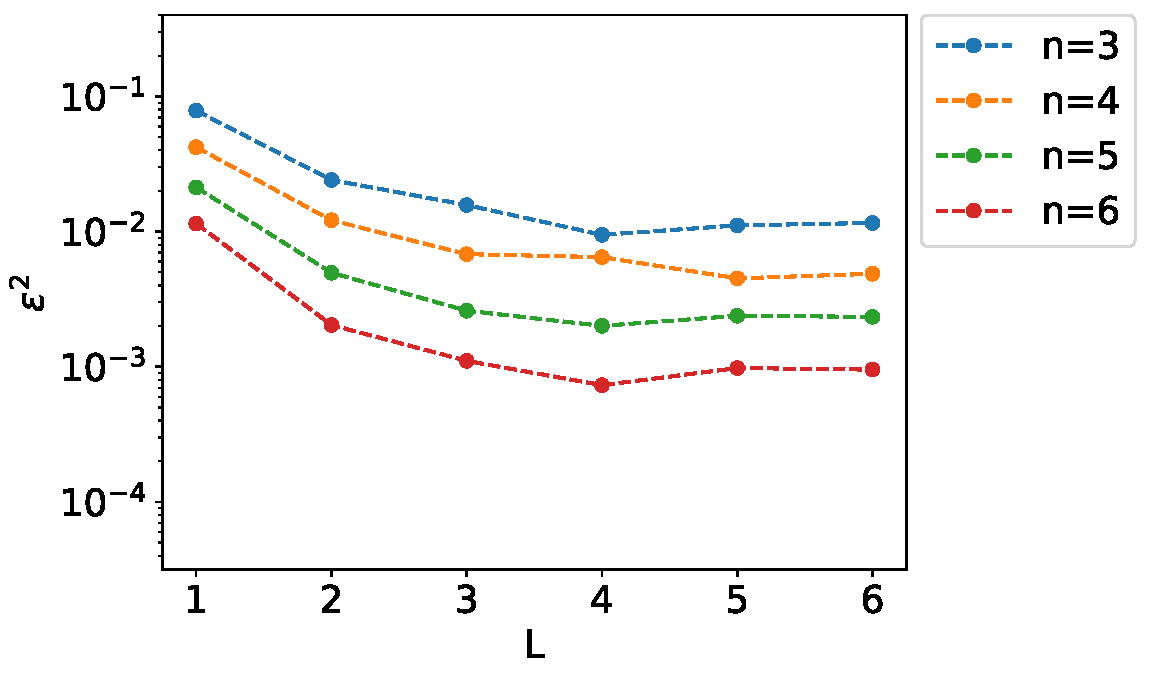
\includegraphics[width=7cm]{product-circuit-exp.pdf}
            \end{figure}
        \end{column}
        
        \begin{column}{0.5\textwidth}
            \centering\hspace*{-30pt} Alternating Layered Ansatz
            \begin{figure}
                \centering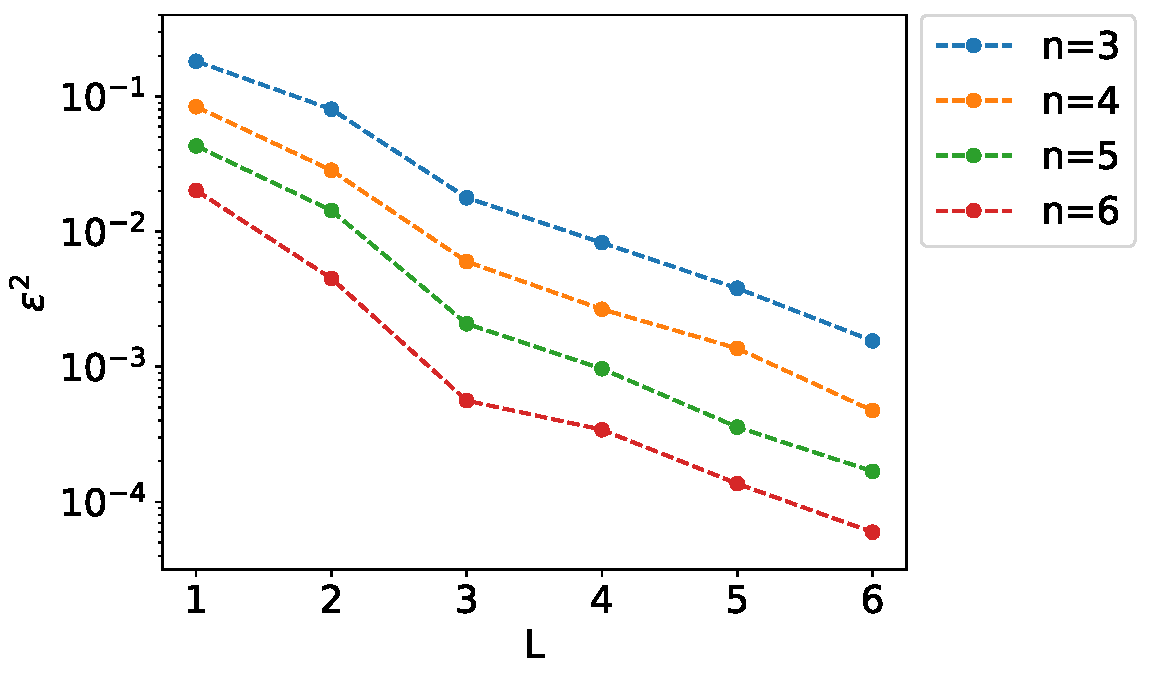
\includegraphics[width=7cm]{alt-circuit-exp.pdf}
            \end{figure}
        \end{column}
    \end{columns}
\end{frame}




\begin{frame}{Explicit Form of the Upper Bound}
    $$
        y_i \in \{0,1\},\quad \colorbox{orange!30}{$\ell_i(\bth)$} := \Tr[\rho_i(\bth)\,O_\rmL] \in [0,1],\quad
        \colorbox{green!30}{$\calL(\bth)$} := \frac1N\sum_{i=1}^N f(y_i, \colorbox{orange!30}{$\ell_i(\bth)$})
    $$
    \begin{theorem}
        Upper bound on the variance of the gradient
        \begin{align*}
            &\Var_{\bth}[\pd_{\theta_\nu} \colorbox{green!30}{$\calL(\bth)$}]\\
            &\leq A_f \times r_{n,s} \times \bar{D}_{\mathrm{HS}}\\
            &=
            2\max_{i,\bth} [(\pd_{\ell_i(\bth)}f)^2]
            \times \frac{2^{2s-1}}{(2^{2s}-1)^2}\qty(\Tr[(O_\rmL^h)^2] - \frac{\Tr[O_\rmL^h]^2}{2^s})
            \times \int_{\bbU}dU D_{\mathrm{HS}} ( \rho^{(h)},\, \bbI/2^s )
        \end{align*}
        , where $O_\rmL^h = \Tr_{\bar{h}}[O_\rmL]$
    \end{theorem}
\end{frame}



\begin{frame}{Ansatz of Slide~\ref{qml-var-alt}}
    \begin{columns}
        \begin{column}{0.5\textwidth}
        Unitary $2$--design of 1-qubit
        \begin{figure}[H]
            \centering
            \begin{tikzpicture}
                \node[scale=1]{
                    \begin{quantikz}
                        \qw & \gate[wires=1,style={fill=red!50}][1cm][0.7cm]{}& \qw
                    \end{quantikz}
                    \begin{quantikz}
                        {\LARGE \textbf{=}}
                    \end{quantikz}
                    \begin{quantikz}
                        \qw\slice{} & \gate{R_x} &\gate{R_y}\slice{$\times 10$} & \qw
                    \end{quantikz}
                    };
            \end{tikzpicture}
            \caption{Structure used as the gate block of TPA}
            \label{fig:tpa-example}
        \end{figure}
        \end{column}
        
        \begin{column}{0.5\textwidth}
            \begin{figure}[H]
                \centering
                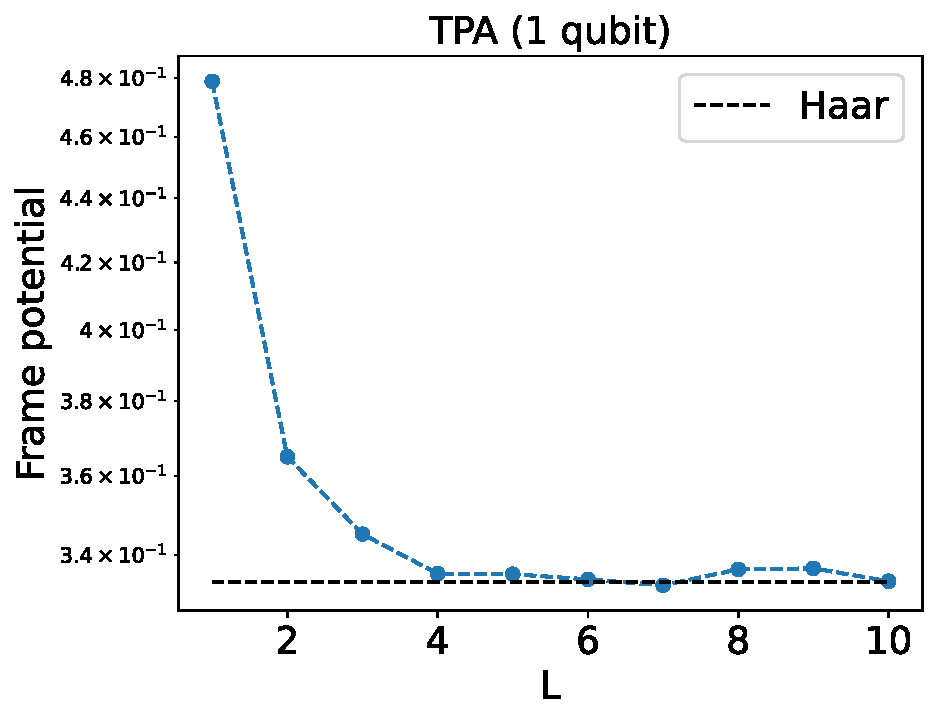
\includegraphics[width=6cm]{1qubit-tpa-exp.pdf}
                \caption{Frame potential of the Tensor Product Ansatz for 1-qubit. The black dashed line represents the frame potential ($=1/3$) when the 1-qubit forms a unitary $2$--design.}
                \label{fig:1qubit-tpa-exp}
            \end{figure}
        \end{column}
    \end{columns}
\end{frame}




\begin{frame}{Lower Bound: Discussion on $\calL_{\mathrm{MAE}}(\bth)$}
    As an extreme example, consider the case where input data belonging to label $0$, $\calX = \{\bs{x}\}$, and input data belonging to label $1$, $\calZ = \{\bs{z}\}$, are such that $\calX = \calZ$.
    In this case,
    \begin{alignat*}{2}
        \calL_{\mathrm{MAE}}(\bth)
        &= \frac1N\Big(\sum_{x\in\calX} |\ell_{i}(\bth) - 0| &&+ \sum_{z\in\calZ} |\ell_{i}(\bth) - 1|\Big)\\
        &= \frac1N\Big(\sum_{x\in\calX} \ell_{i}(\bth)       &&+ \sum_{x\in\calX} (1 - \ell_{i}(\bth))\Big) = \frac12
    \end{alignat*}
    
    Therefore, the gradient of the cost function becomes $0$, and so does the variance.\\
    → Even if the structure of the encoding circuit is extremely simple, the closer the input data between different labels are, the smaller the variance of the gradient becomes.
\end{frame}

\begin{frame}{Lower Bound: Discussion on $\calL_{\mathrm{MSE}}(\bth)$}
    As an extreme example, consider the case where input data belonging to label $0$, $\calX = \{\bs{x}\}$, and input data belonging to label $1$, $\calZ = \{\bs{z}\}$, are such that $\calX = \calZ$.
    In this case,
    \begin{alignat*}{2}
        \calL_{\mathrm{MSE}}(\bth)
        &= \frac1N\Big(\sum_{x\in\calX} (\ell_{i} - 0)^2 &+ \sum_{x\in\calX} (\ell_{i} - 1)^2\Big)\\
        &= \frac1N\Big(\sum_{x\in\calX} \ell_{i}^2       &+ \sum_{x\in\calX} (\ell_{i} - 1)^2\Big)\\
        &= \frac12 + \frac1N\sum_{x\in\calX} 2\qty(\ell_i - \frac12)^2
    \end{alignat*}
    
    In this case, since the cost function $\calL_{\mathrm{MSE}}(\bth)$ is minimized when $\ell_i$ is $\frac12$, it never approaches the ground truth labels $y_i = \{0,1\}$.
\end{frame}

\begin{frame}{Lower Bound: Discussion on $\calL_{\mathrm{LOG}}(\bth)$}
    As an extreme example, consider the case where input data belonging to label $0$, $\calX = \{\bs{x}\}$, and input data belonging to label $1$, $\calZ = \{\bs{z}\}$, are such that $\calX = \calZ$.
    In this case,
    \begin{align*}
        \calL_{\mathrm{LOG}}(\bth)
        &= \frac1N\Big(\sum_{x\in\calX} -\log(1-\ell_i) + \sum_{x\in\calX} -\log(\ell_i)\Big)\\
        &= \frac1N\Big(\sum_{x\in\calX} - \log\ell_i(1-\ell_i)\Big)\\
        &= \frac1N\Big(\sum_{x\in\calX} - \log\qty[-\qty(\ell_i - \frac12)^2 + \frac14]\Big)
    \end{align*}
    
    In this case, since the cost function $\calL_{\mathrm{LOG}}(\bth)$ is minimized when $\ell_i$ is $\frac12$, it never approaches the ground truth labels $y_i = \{0,1\}$.
\end{frame}




\end{document}
